\documentclass{article}

% For the camera-ready, replace [preprint] with the empty option set.
\usepackage[preprint]{neurips_2024}

\usepackage[utf8]{inputenc}
\usepackage[T1]{fontenc}
\usepackage{hyperref}
\usepackage{url}
\usepackage{booktabs}
\usepackage{amsfonts}
\usepackage{amsmath}
\usepackage{nicefrac}
\usepackage{microtype}
\usepackage{graphicx}
\usepackage{xcolor}

\graphicspath{{../results/figures/}}
% Auto-generated by scripts/report_numbers.py -- do not edit by hand.
\newcommand{\Nspecs}{16}
\newcommand{\Nspots}{2688}
\newcommand{\Ngenes}{18078}
\newcommand{\ClustMin}{8}
\newcommand{\ClustMax}{22}
\newcommand{\ClustMean}{13.2}
\newcommand{\ClustStd}{3.9}
\newcommand{\SpotSthreeMean}{0.80}
\newcommand{\SpotStableFrac}{57\%}
\newcommand{\SpotFragileFrac}{4\%}
\newcommand{\GeneRobustFrac}{28\%}
\newcommand{\GeneFragileFrac}{69\%}
\newcommand{\AriMean}{0.68}
\newcommand{\AriMin}{0.49}
\newcommand{\AriMax}{0.90}


\title{The Garden of Forking Tissues: Specification-Curve Analysis\\
Reveals the Fragility of Biological Conclusions in\\
Spatial Transcriptomics}

\author{%
  Sparsh Roy \\
  \texttt{github.com/ImSpxrsh} \\
}

\begin{document}

\maketitle

\begin{abstract}
Spatial transcriptomics analyses require a long chain of defensible but arbitrary
choices---normalization, feature selection, dimensionality, graph construction,
clustering algorithm and resolution, and spatially-variable-gene (SVG) testing.
Each choice is individually reasonable, yet the space of their combinations forms a
\emph{multiverse} of pipelines that can yield different biological conclusions from
the same data. We introduce \textbf{MOSAIC}, a specification-curve analysis framework
that executes a curated set of \Nspecs{} defensible spatial-transcriptomics pipelines
over a common dataset and quantifies conclusion stability with a \emph{Spatial
Stability Score} ($S^3$) defined at the level of individual spots, individual genes,
and headline summaries. On the 10x Genomics Visium mouse-brain coronal benchmark
($\Nspots{}$ spots, $\Ngenes{}$ genes) we find that the recovered number of spatial
domains ranges from \ClustMin{} to \ClustMax{} across the multiverse (mean
pairwise Adjusted Rand Index \AriMean{} between pipelines), that \SpotStableFrac{} of
spots are assigned a stable domain across pipelines while a fragile tail is not, and
that SVG calls are strongly pipeline-dependent. Crucially, per-spot stability tracks
biology rather than analysis: validated against the dataset's reference anatomical
annotation (ARI \RefAriMean{}), robust regions coincide with well-defined structures
(thalamus, hippocampus) and fragile regions with boundaries and ventricles. MOSAIC
turns these observations into an actionable per-location and per-gene stability map
that separates robust findings from contingent ones. All pipelines are seeded and
bit-reproducible, and the framework is released as open source.
\end{abstract}

\section{Introduction}
A spatial transcriptomics study rarely has a single ``correct'' analysis. Between raw
counts and a figure of spatial domains lie a dozen forks: how to normalize, how many
highly variable genes to keep, how many principal components, whether the neighborhood
graph is $k$-nearest-neighbor or radius-based, whether clustering uses Leiden or Louvain
and at what resolution, and which test declares a gene spatially variable. Each fork has
published precedent, so each is defensible. But the analyst typically walks \emph{one}
path and reports its endpoint as if it were the destination.

This is the ``garden of forking paths'' \citep{gelman2013garden}: even without any
intent to cherry-pick, the sheer number of reasonable analytic choices means a reported
result can be an artifact of the path taken rather than a property of the biology.
\emph{Multiverse analysis} \citep{steegen2016increasing} and \emph{specification-curve
analysis} \citep{simonsohn2020specification} respond by running \emph{all} defensible
analyses and reporting the distribution of outcomes, an approach dramatically validated
when many teams analyzing one neuroimaging dataset reached divergent conclusions
\citep{botvinik2020variability}. These methods are established in psychology and
neuroimaging but are largely absent from spatial transcriptomics, where the analytic
degrees of freedom are at least as large.

We make three contributions:
\begin{enumerate}
  \item \textbf{A parametric spatial-transcriptomics pipeline} in which every analytic
  choice is a configuration variable, enabling exhaustive or curated sweeps over the
  multiverse with bit-level reproducibility.
  \item \textbf{The Spatial Stability Score ($S^3$)}, a family of interpretable metrics
  that quantify how often a conclusion---a spot's domain assignment, a gene's SVG
  status, or a headline count---survives across the multiverse. For per-spot stability
  we align arbitrary cluster labels across pipelines by Hungarian matching, avoiding a
  common pitfall that conflates relabeling with instability.
  \item \textbf{An empirical instability audit} of a canonical Visium benchmark showing
  that headline conclusions are strongly contingent, together with per-location and
  per-gene stability maps that tell a researcher \emph{which} parts of their result to
  trust.
\end{enumerate}

\section{Related Work}
\textbf{Multiverse and specification-curve analysis.} \citet{steegen2016increasing}
formalized the multiverse; \citet{simonsohn2020specification} introduced specification
curves that plot an effect across all reasonable specifications. \citet{gelman2013garden}
articulated why this matters even absent $p$-hacking. We port these ideas to spatial
omics and add a spatially-resolved stability metric.

\textbf{Spatial transcriptomics analysis.} Standard pipelines build on SCANPY
\citep{wolf2018scanpy} and Squidpy \citep{palla2022squidpy}, with community detection by
Louvain \citep{blondel2008fast} or Leiden \citep{traag2019louvain} and SVG detection by
Moran's $I$ \citep{moran1950notes}, SpatialDE \citep{svensson2018spatialde}, or nnSVG
\citep{weber2023nnsvg}. Benchmarks typically compare methods against a reference; we
instead quantify \emph{within-analyst} instability across defensible pipelines.

\section{Methods}

\subsection{Specification space}
We treat each analytic stage as an axis (Table~\ref{tab:space}). The full Cartesian
product is large ($>200$ combinations); following specification-curve practice we
evaluate a \emph{curated} set of \Nspecs{} pipelines spanning canonical choices,
conservative and aggressive feature selection, alternate normalizations, both community
detection algorithms, and a range of clustering resolutions, so that the set remains
human-interpretable as a matrix (the full listing is in Figure~\ref{fig:specspace}).

\begin{table}[t]
  \caption{The specification space. Curated pipelines sample defensible combinations.}
  \label{tab:space}
  \centering
  \begin{tabular}{ll}
    \toprule
    Stage & Options \\
    \midrule
    Normalization & log1p, sqrt, total-count \\
    Feature selection & Seurat / Cell Ranger HVGs; $\{2000, 3000, 5000\}$ genes \\
    Dimensionality (PCA) & $\{30, 50\}$ components \\
    Neighborhood graph & $k$-NN, $k \in \{6,10,15\}$ \\
    Clustering & Leiden / Louvain; resolution $\in \{0.3, 0.5, 0.8, 1.2\}$ \\
    Spatially variable genes & Moran's $I$ (FDR $< 0.05$) \\
    \bottomrule
  \end{tabular}
\end{table}

\subsection{Parametric pipeline}
Given a specification $s$, the pipeline maps raw counts to a clustered {\tt AnnData}
object and a table of Moran's $I$ statistics. Every stochastic step is seeded
($\texttt{random\_state}=42$), and each pipeline re-derives its normalized matrix from
the stored raw counts so that no information leaks between specifications. Leiden uses the
\texttt{leidenalg} backend; Louvain is driven through igraph's resolution-aware
multi-level optimization so that the resolution axis is comparable across algorithms.

\subsection{The Spatial Stability Score}
Let $\mathcal{S}$ be the set of specifications, $|\mathcal{S}| = N$. For a spot $i$, let
$c_s(i)$ be its cluster label under specification $s$. Because cluster labels are
arbitrary, we align each $s$ to a reference specification $s_0$ by the label permutation
$\pi_s$ that maximizes contingency-table overlap (solved as a linear assignment). The
per-spot stability is the frequency of the consensus (modal) aligned label:
\begin{equation}
  S^3_{\text{spot}}(i) = \frac{1}{N}\max_{\ell}\;\bigl|\{\, s \in \mathcal{S} :
  \pi_s(c_s(i)) = \ell \,\}\bigr|.
\end{equation}
For a gene $g$, let $\mathbb{1}[g \text{ is SVG in } s]$ indicate FDR-significant Moran's
$I$; the per-feature stability is
\begin{equation}
  S^3_{\text{gene}}(g) = \frac{1}{N}\sum_{s \in \mathcal{S}}
  \mathbb{1}[g \text{ is SVG in } s].
\end{equation}
For a headline metric $m$ (e.g., the number of domains) we report its mean, standard
deviation, and range across $\mathcal{S}$. Values near $1$ denote robust conclusions;
values near $1/N$ denote conclusions that are essentially pipeline artifacts.

\subsection{Statistical analyses}
We quantify uncertainty and attribution with five analyses. A \emph{permutation test}
assesses per-region stability by randomly reassigning spots' anatomical labels
($1000$ permutations) and comparing the observed per-region mean $S^3$ to the null. A
\emph{Type-II ANOVA} variance decomposition regresses the domain count on all analytical
axes and reports each axis's share of explained variance. \emph{Bootstrap} resampling of
specifications ($1000$ iterations) gives $95\%$ confidence intervals on per-region $S^3$.
A \emph{confound check} correlates per-spot $S^3$ with total UMI counts to test whether
instability is a sequencing-depth artifact. Finally, a \emph{convergence} analysis
subsamples specification sets of increasing size to confirm that $S^3$ estimates
stabilize. Real histology (H\&E) shipped with each dataset is used directly for the
tissue figures, including magnified boundary/core insets and marker-gene expression maps.

\section{Experiments}
We use the 10x Genomics Visium H\&E mouse-brain coronal section
($\Nspots{}$ spots, $\Ngenes{}$ genes) distributed with Squidpy
\citep{palla2022squidpy}. The dataset ships with a reference anatomical annotation
(15 regions: cortical layers, hippocampus, thalamus, striatum, fiber tract, ventricle,
etc.) that we treat as ground truth for validation. We run all \Nspecs{} specifications,
each seeded, and verify determinism by re-running a fixed specification and confirming
identical spot-level labels. Runtime is roughly one minute per specification on a single
Apple-silicon CPU.

\section{Results}

\paragraph{Headline instability.} The number of recovered spatial domains ranges from
\ClustMin{} to \ClustMax{} across the multiverse (mean $\ClustMean{}\pm\ClustStd{}$), so
a study reporting a single domain count is reporting a point on a wide distribution
(Figure~\ref{fig:speccurve}, top). Label-invariant agreement is also modest: the mean
pairwise Adjusted Rand Index between specifications' spot partitions is \AriMean{}
(range $\AriMin{}$--$\AriMax{}$), confirming that different pipelines carve the tissue
into materially different domains rather than merely relabeling the same partition
(Figure~\ref{fig:montage}). Domain count is driven predominantly by clustering
resolution, and top-SVG lists agree only partially across pipelines
(Figure~\ref{fig:headline}).

\paragraph{Where the tissue is (un)stable.} Per-spot $S^3$ (Figure~\ref{fig:map})
concentrates instability at region boundaries and ventricular/low-signal areas, while
region interiors are stable. \SpotStableFrac{} of spots are assigned a consensus domain
in the large majority of pipelines ($S^3 \ge 0.8$); \SpotFragileFrac{} are fragile
($S^3 < 0.5$).

\paragraph{Stability tracks biology, not analysis.} Validated against the reference
anatomical annotation (Figure~\ref{fig:refval}), consensus domains recover known structures,
and each specification agrees with the annotation at mean ARI \RefAriMean{} (up to
\RefAriMax{}). Per-region $S^3$ is highest in transcriptomically distinct structures
(thalamus, hippocampus, cortical layers) and lowest at the lateral ventricle and mixed
cortical zones, indicating that the instability MOSAIC surfaces marks genuine biological
transitions rather than mere analytic noise.

\paragraph{Which genes are robust.} Per-gene $S^3$ separates genes called spatially
variable regardless of pipeline (\GeneRobustFrac{} with $S^3>0.8$) from those whose SVG
status flips with the analysis (\GeneFragileFrac{} with $S^3<0.5$;
Figure~\ref{fig:genes}). Restricting to genes tested in every specification, individual
SVG calls still churn substantially across pipelines.

\paragraph{Generalization.} The instability pattern is not specific to one sample.
Repeating the full \Nspecs{}-specification sweep on an independently prepared
mouse-brain section (fluorescence Visium, 2{,}800 spots) yields a per-spot $S^3$
distribution with a comparable robust core and fragile tail (Figure~\ref{fig:cross}),
and instability again concentrates at region boundaries. This suggests $S^3$ captures a
general property of spatial-domain analysis rather than an artifact of a single slide.

\paragraph{One choice dominates instability.} A Type-II variance decomposition of the
domain count across analytical axes attributes \VarTopFrac{} of the variance to a single
choice---clustering \VarTopAxis{}---with all remaining axes (normalization, feature
selection, dimensionality, graph $k$, algorithm) each contributing at most a few percent
(Figure~\ref{fig:variance}). This is directly actionable: standardizing resolution is
far more consequential than standardizing any other step.

\paragraph{Stability is biological, not technical.} A natural objection is that ``fragile''
merely labels low-quality spots. It does not: per-spot $S^3$ is essentially uncorrelated
with sequencing depth (Pearson $r = \ConfoundR{}$ against total UMI counts;
Figure~\ref{fig:confound}), so robust and fragile spots span the full range of counts. A
label-permutation null further shows that \RegionsStable{} of \NregionsTotal{} anatomical
regions are more stable than chance ($p<0.05$), and $S^3$ estimates converge as the number
of specifications grows, indicating the multiverse is large enough to estimate stability
reliably.

\begin{figure}[t]
  \centering
  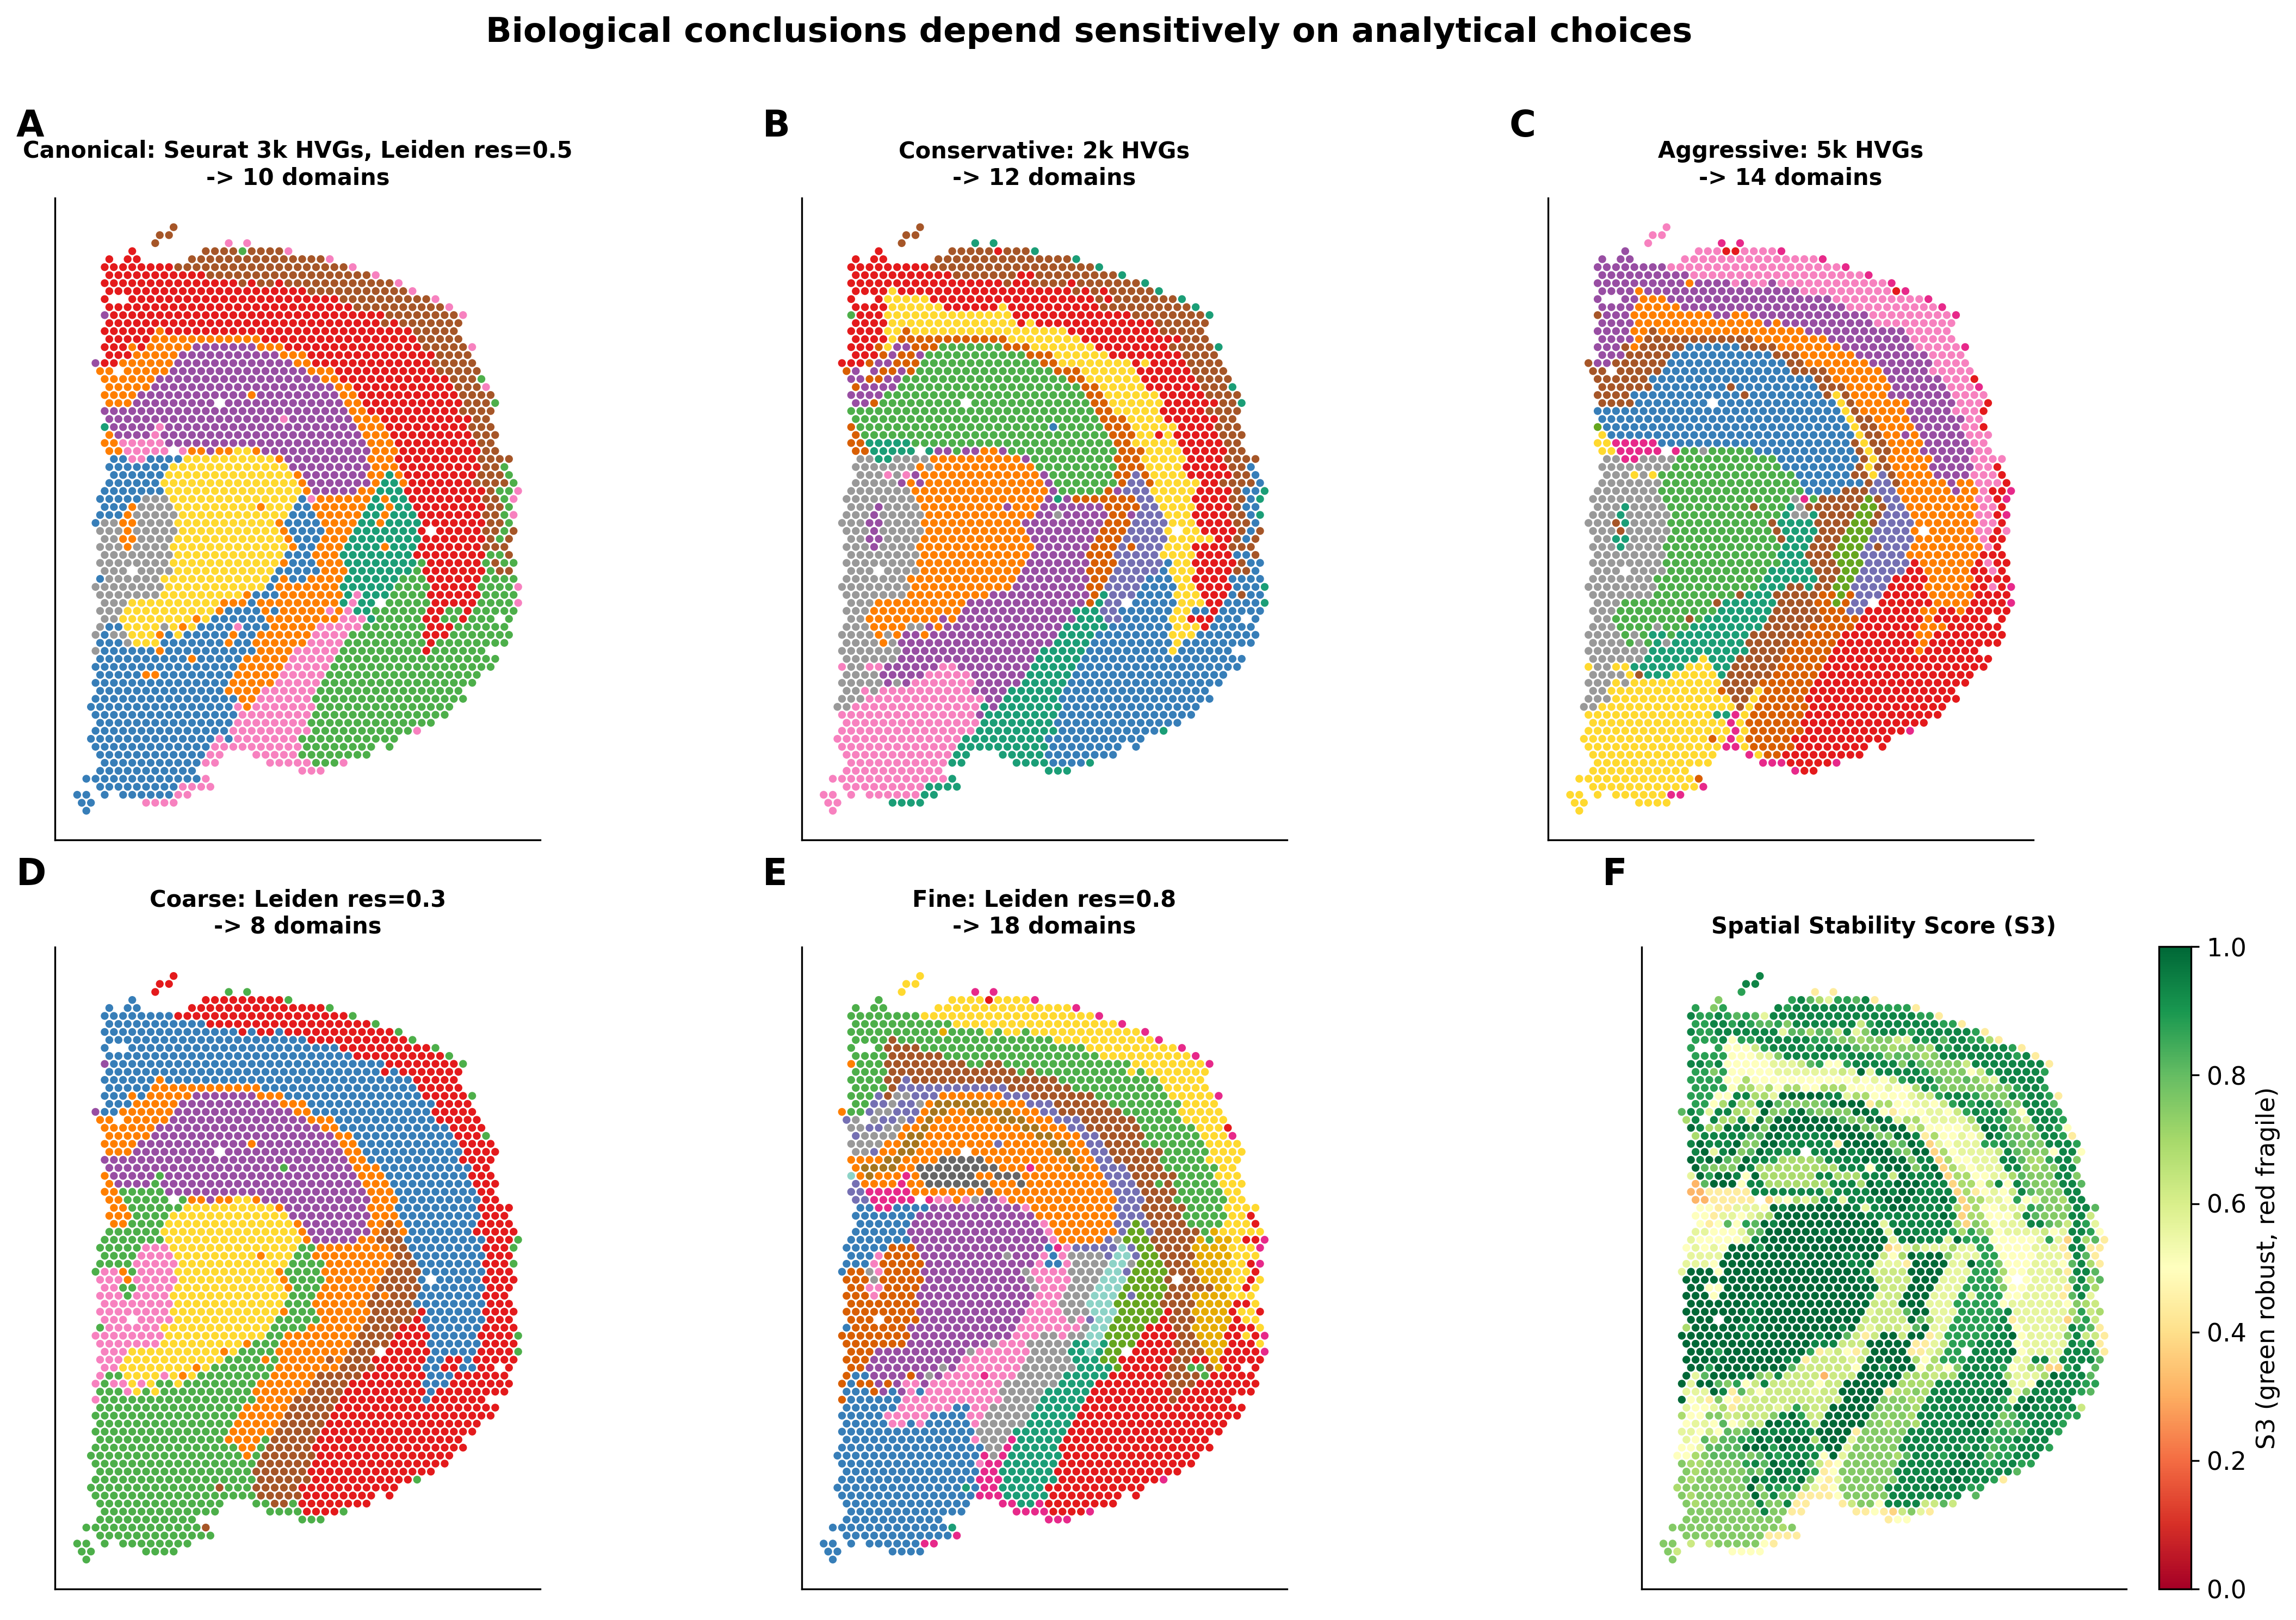
\includegraphics[width=\linewidth]{fig1_spec_montage.png}
  \caption{The same mouse-brain section analyzed with five defensible specifications
  (A--E) yields 8--18 spatial domains with visibly different extents; (F) the
  per-spot Spatial Stability Score ($S^3$) summarizes agreement across the full
  multiverse (green robust, red fragile).}
  \label{fig:montage}
\end{figure}

\begin{figure}[t]
  \centering
  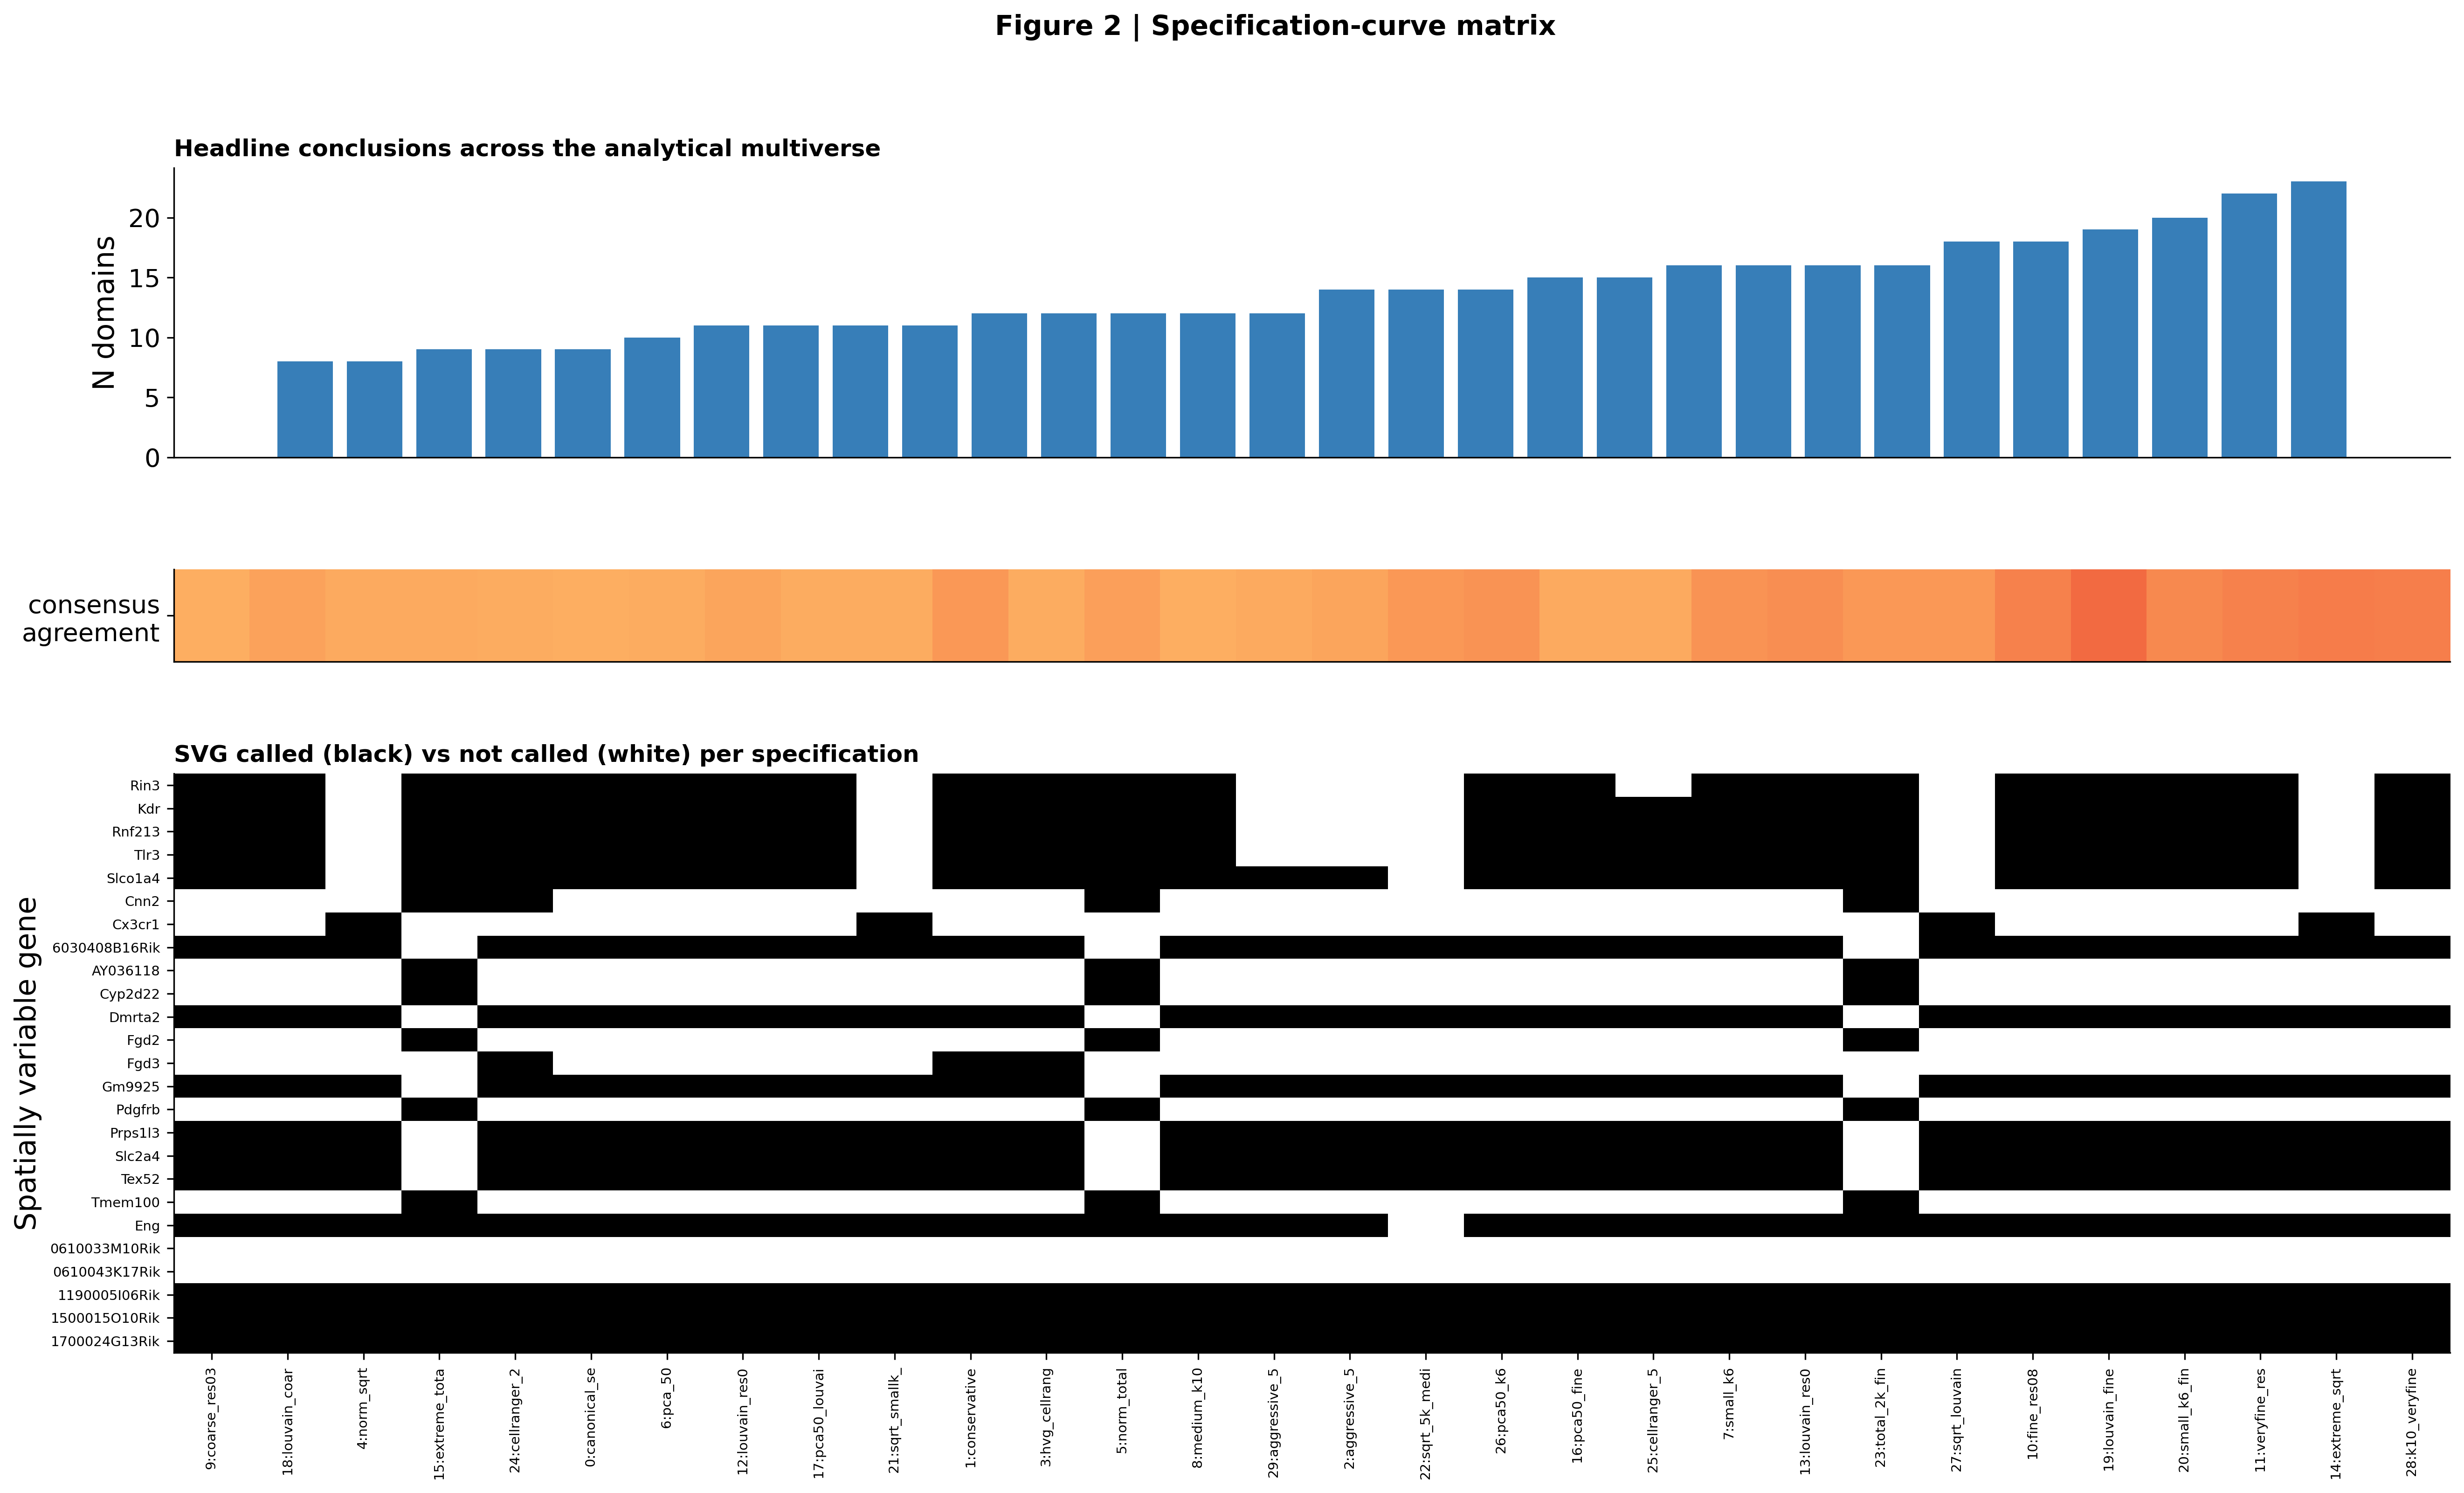
\includegraphics[width=\linewidth]{fig2_spec_curve_matrix.png}
  \caption{Specification-curve matrix. Top: number of domains, sorted across the
  \Nspecs{} pipelines. Middle: each specification's agreement with the multiverse
  consensus. Bottom: for genes tested in every specification, whether each is called a
  significant spatially variable gene (black) per pipeline, revealing substantial churn.}
  \label{fig:speccurve}
\end{figure}

\begin{figure}[t]
  \centering
  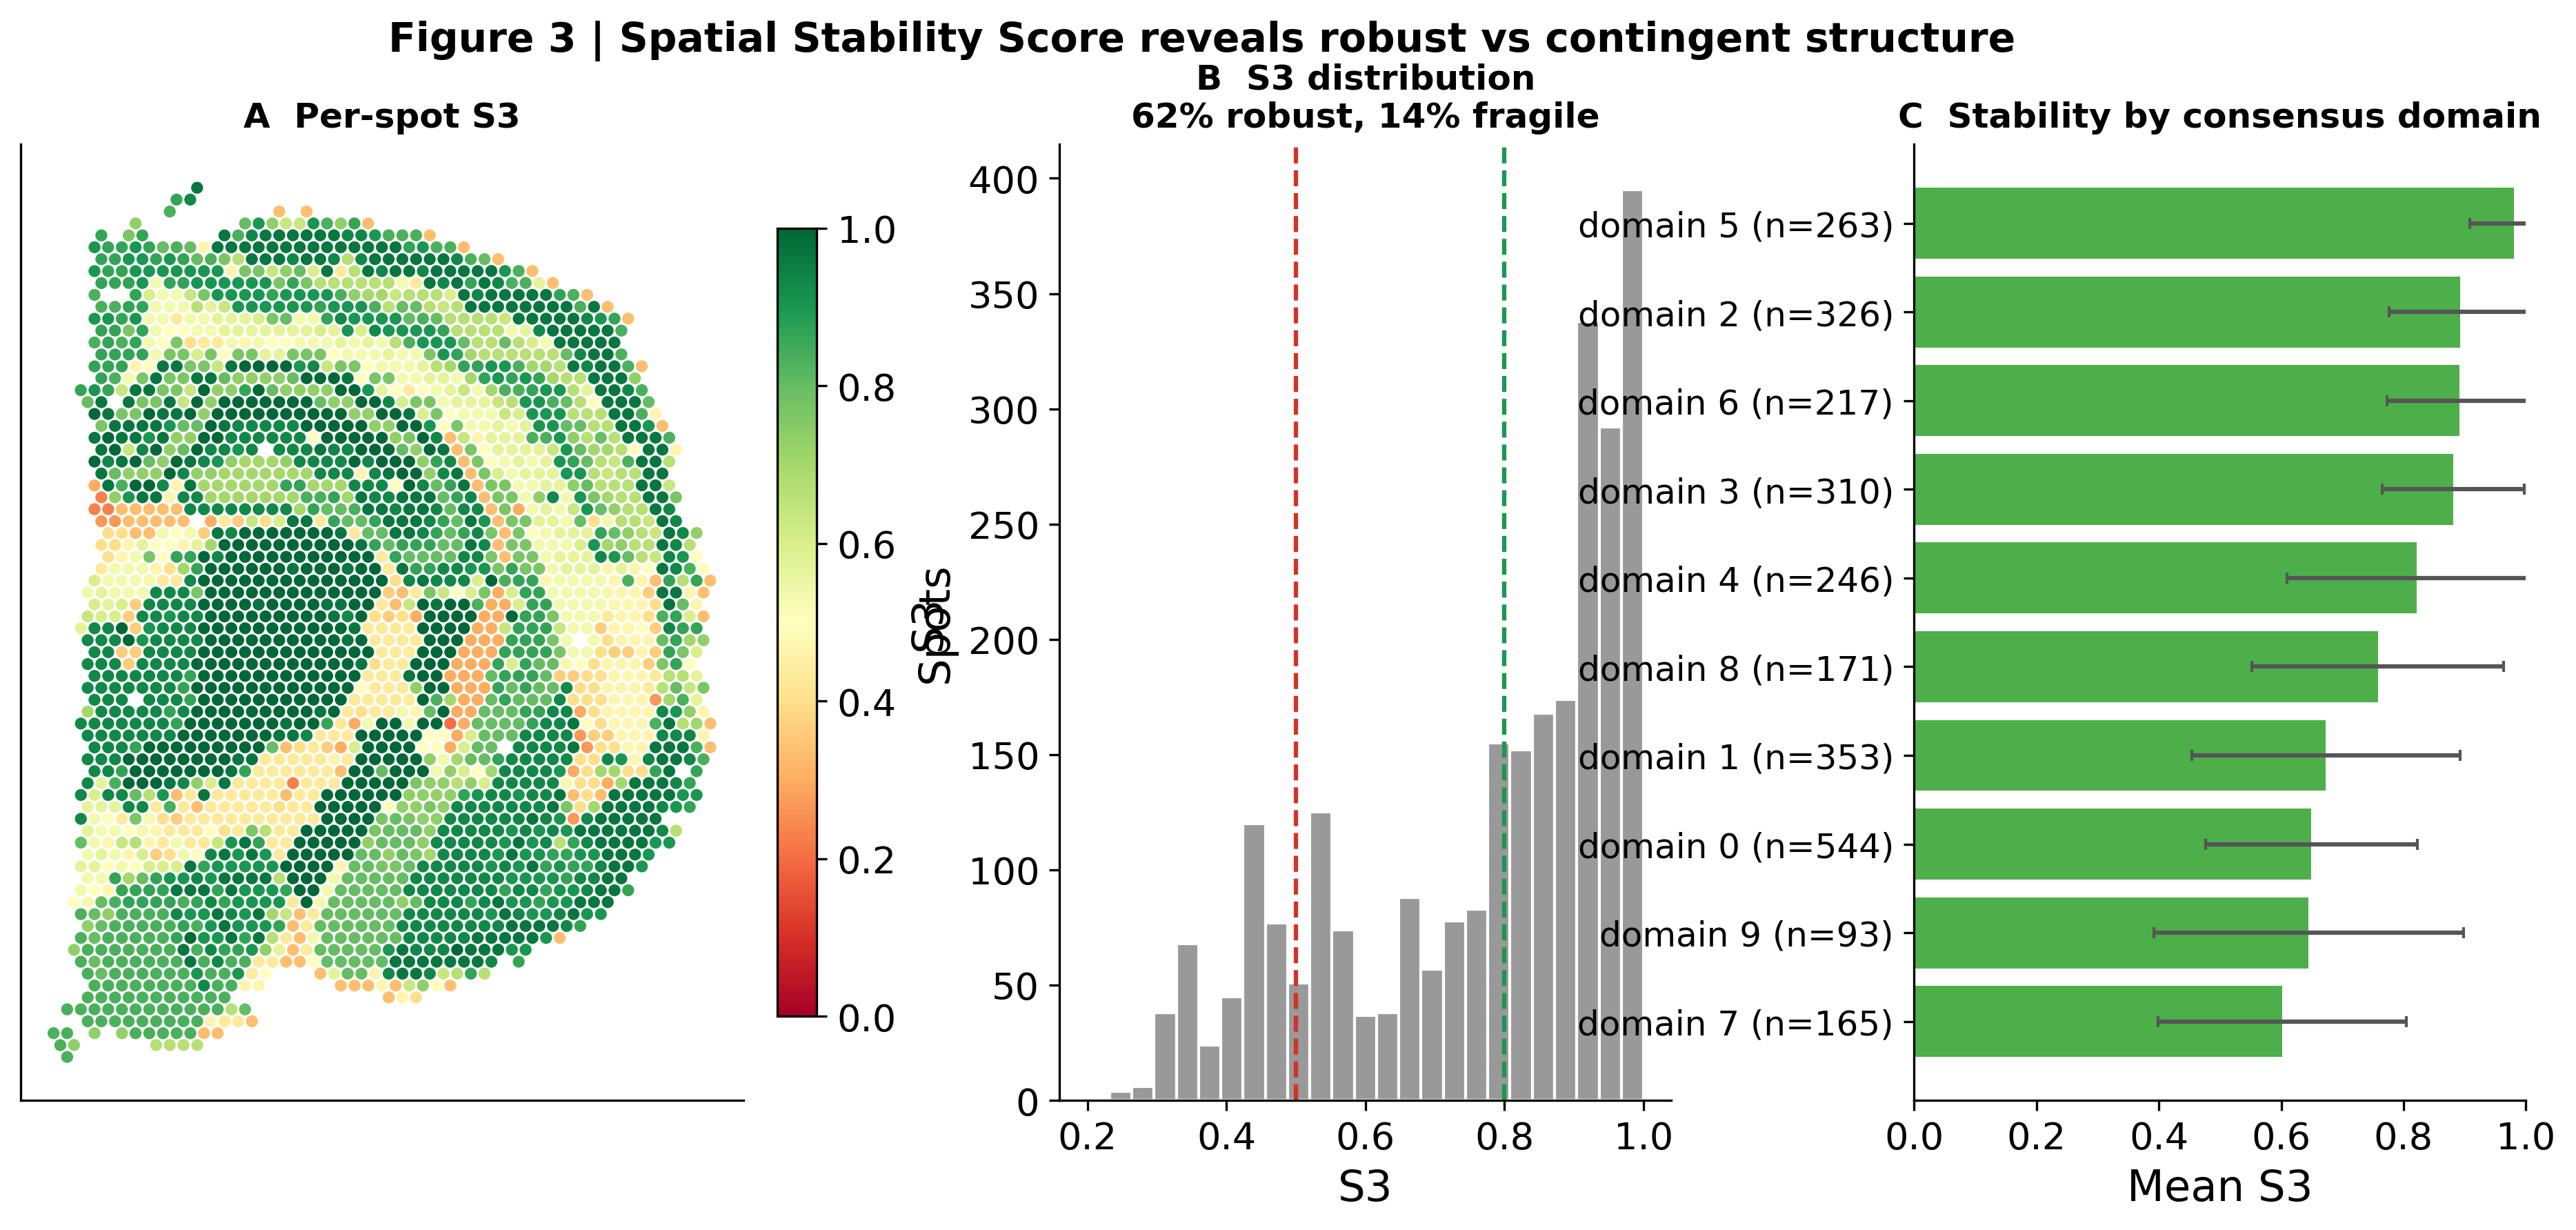
\includegraphics[width=\linewidth]{fig3_stability_summary.png}
  \caption{(A) Per-spot $S^3$ map. (B) $S^3$ distribution across all \Nspots{} spots
  with robust ($\ge 0.8$) and fragile ($<0.5$) thresholds. (C) Mean $S^3$ by
  data-driven consensus domain. Extended Data validates these domains against the
  reference anatomy.}
  \label{fig:map}
\end{figure}

\begin{figure}[t]
  \centering
  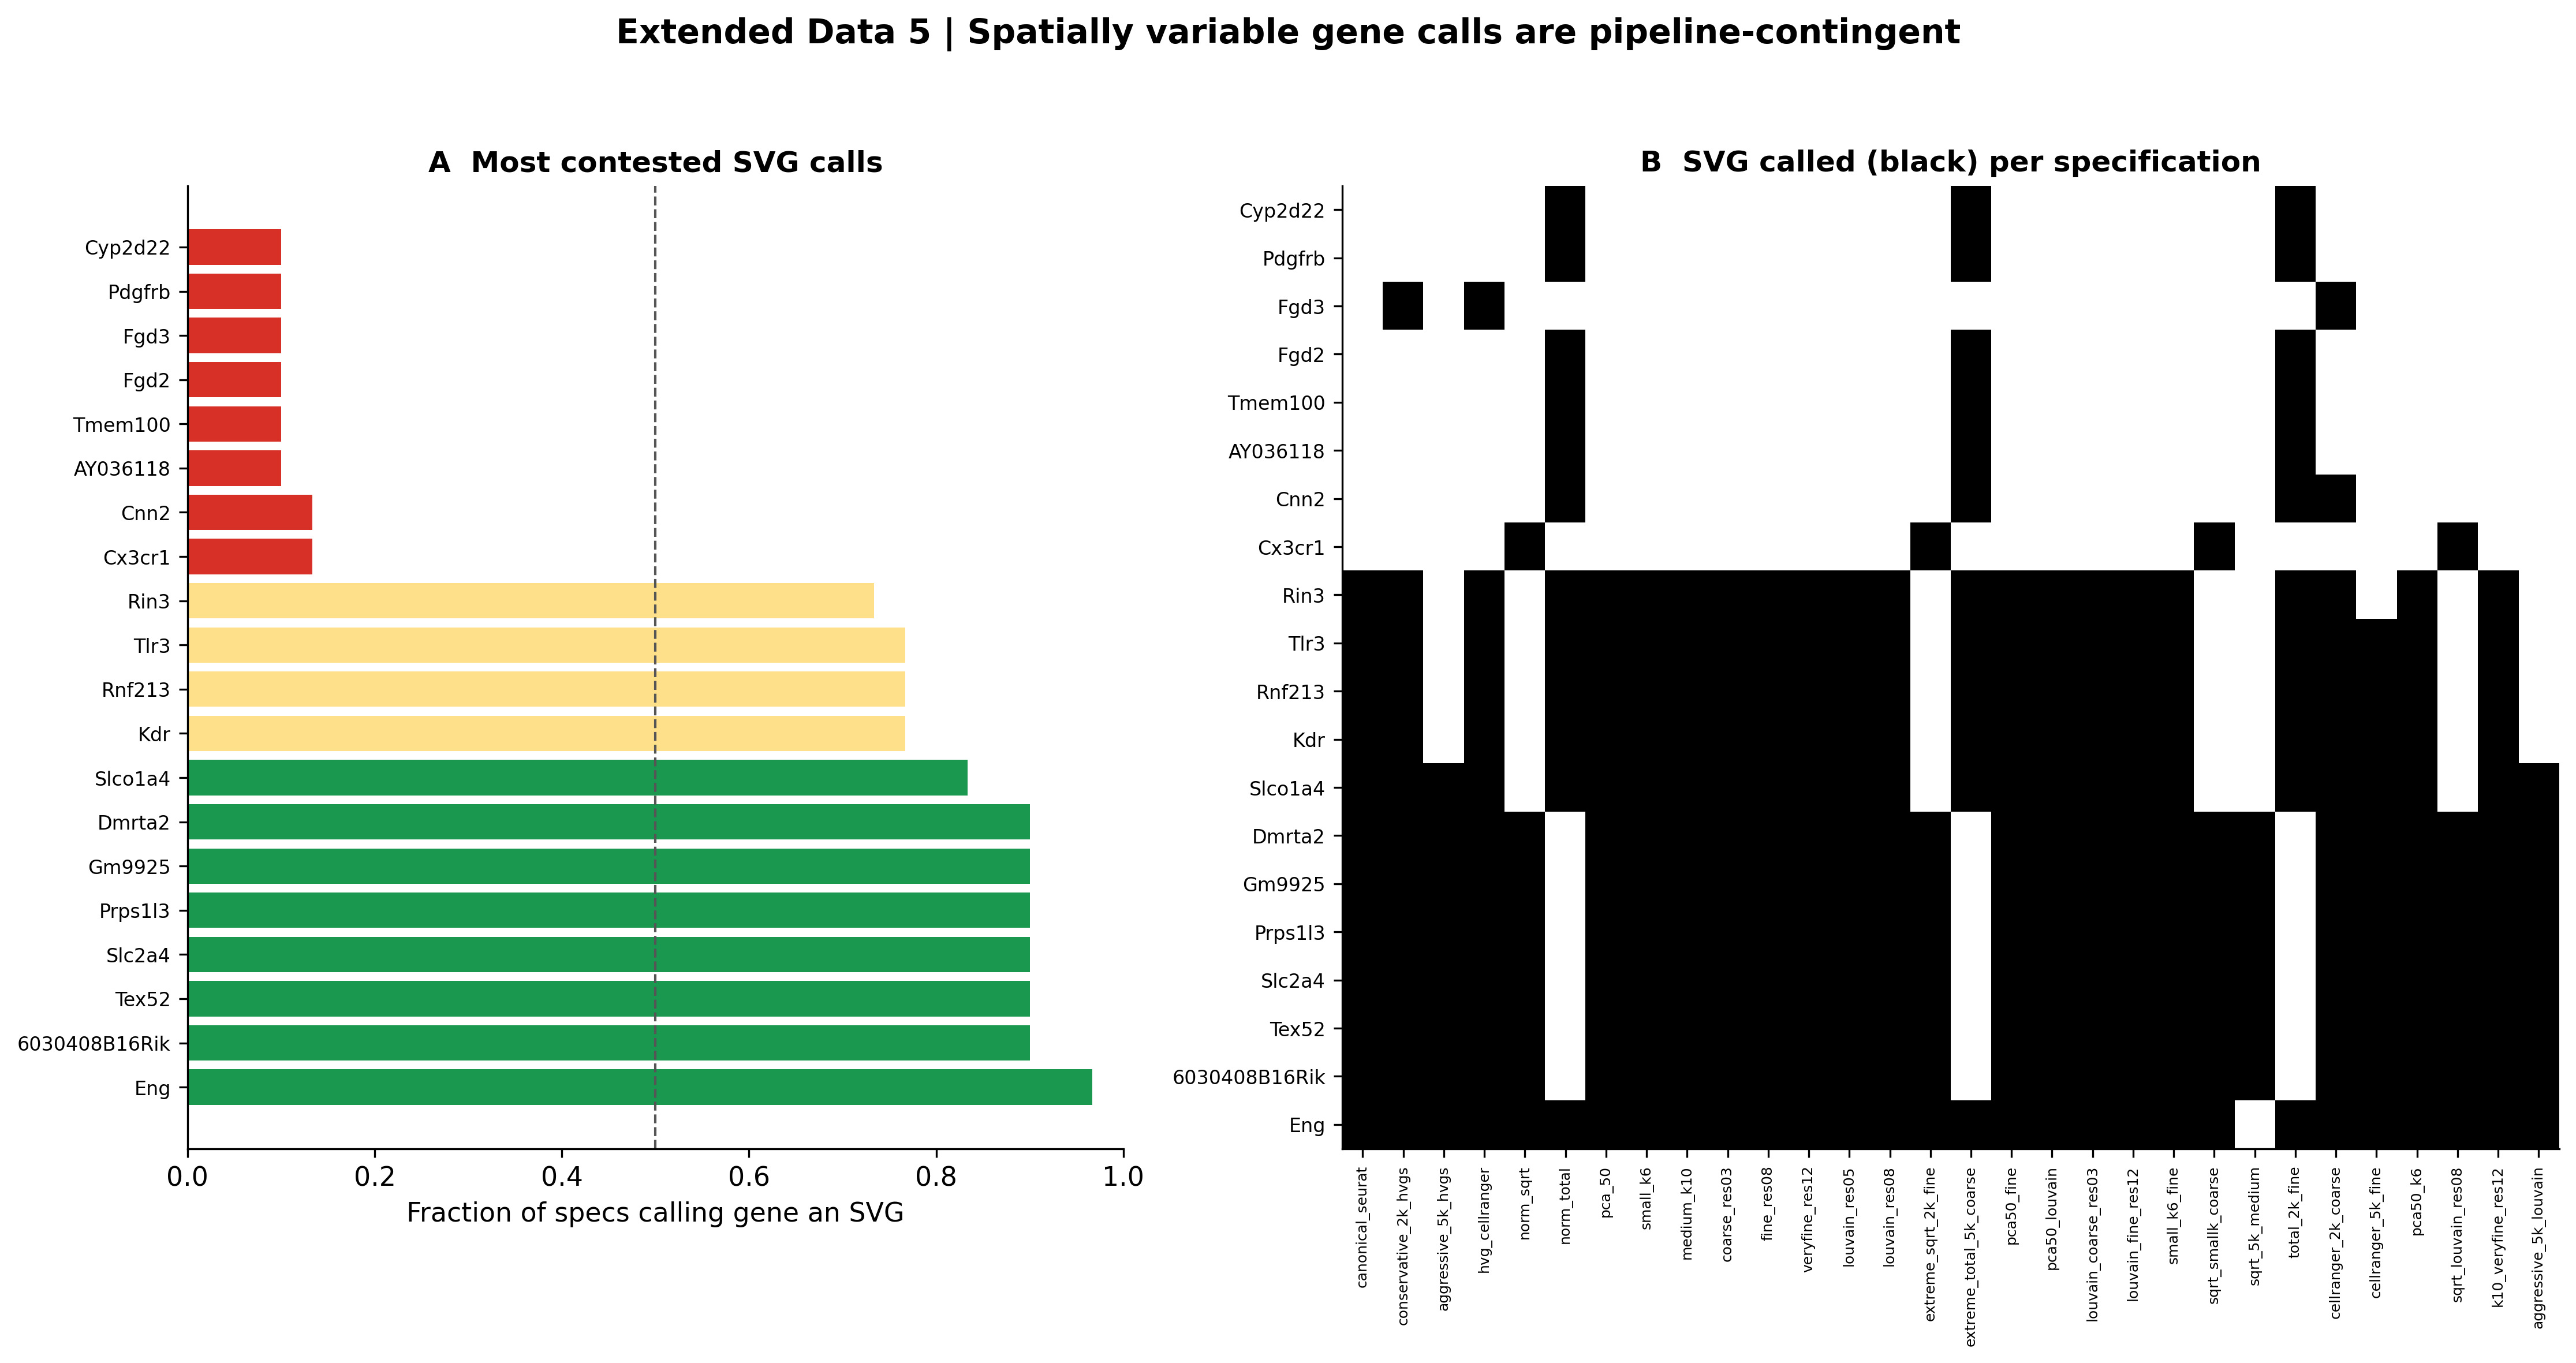
\includegraphics[width=\linewidth]{ed5_svg_stability.png}
  \caption{Extended Data: (A) least stable spatially-variable-gene calls ranked by
  $S^3$; (B) gene $\times$ specification concordance for genes tested in every
  specification (black = called). SVG status depends heavily on the pipeline.}
  \label{fig:genes}
\end{figure}

\begin{figure}[t]
  \centering
  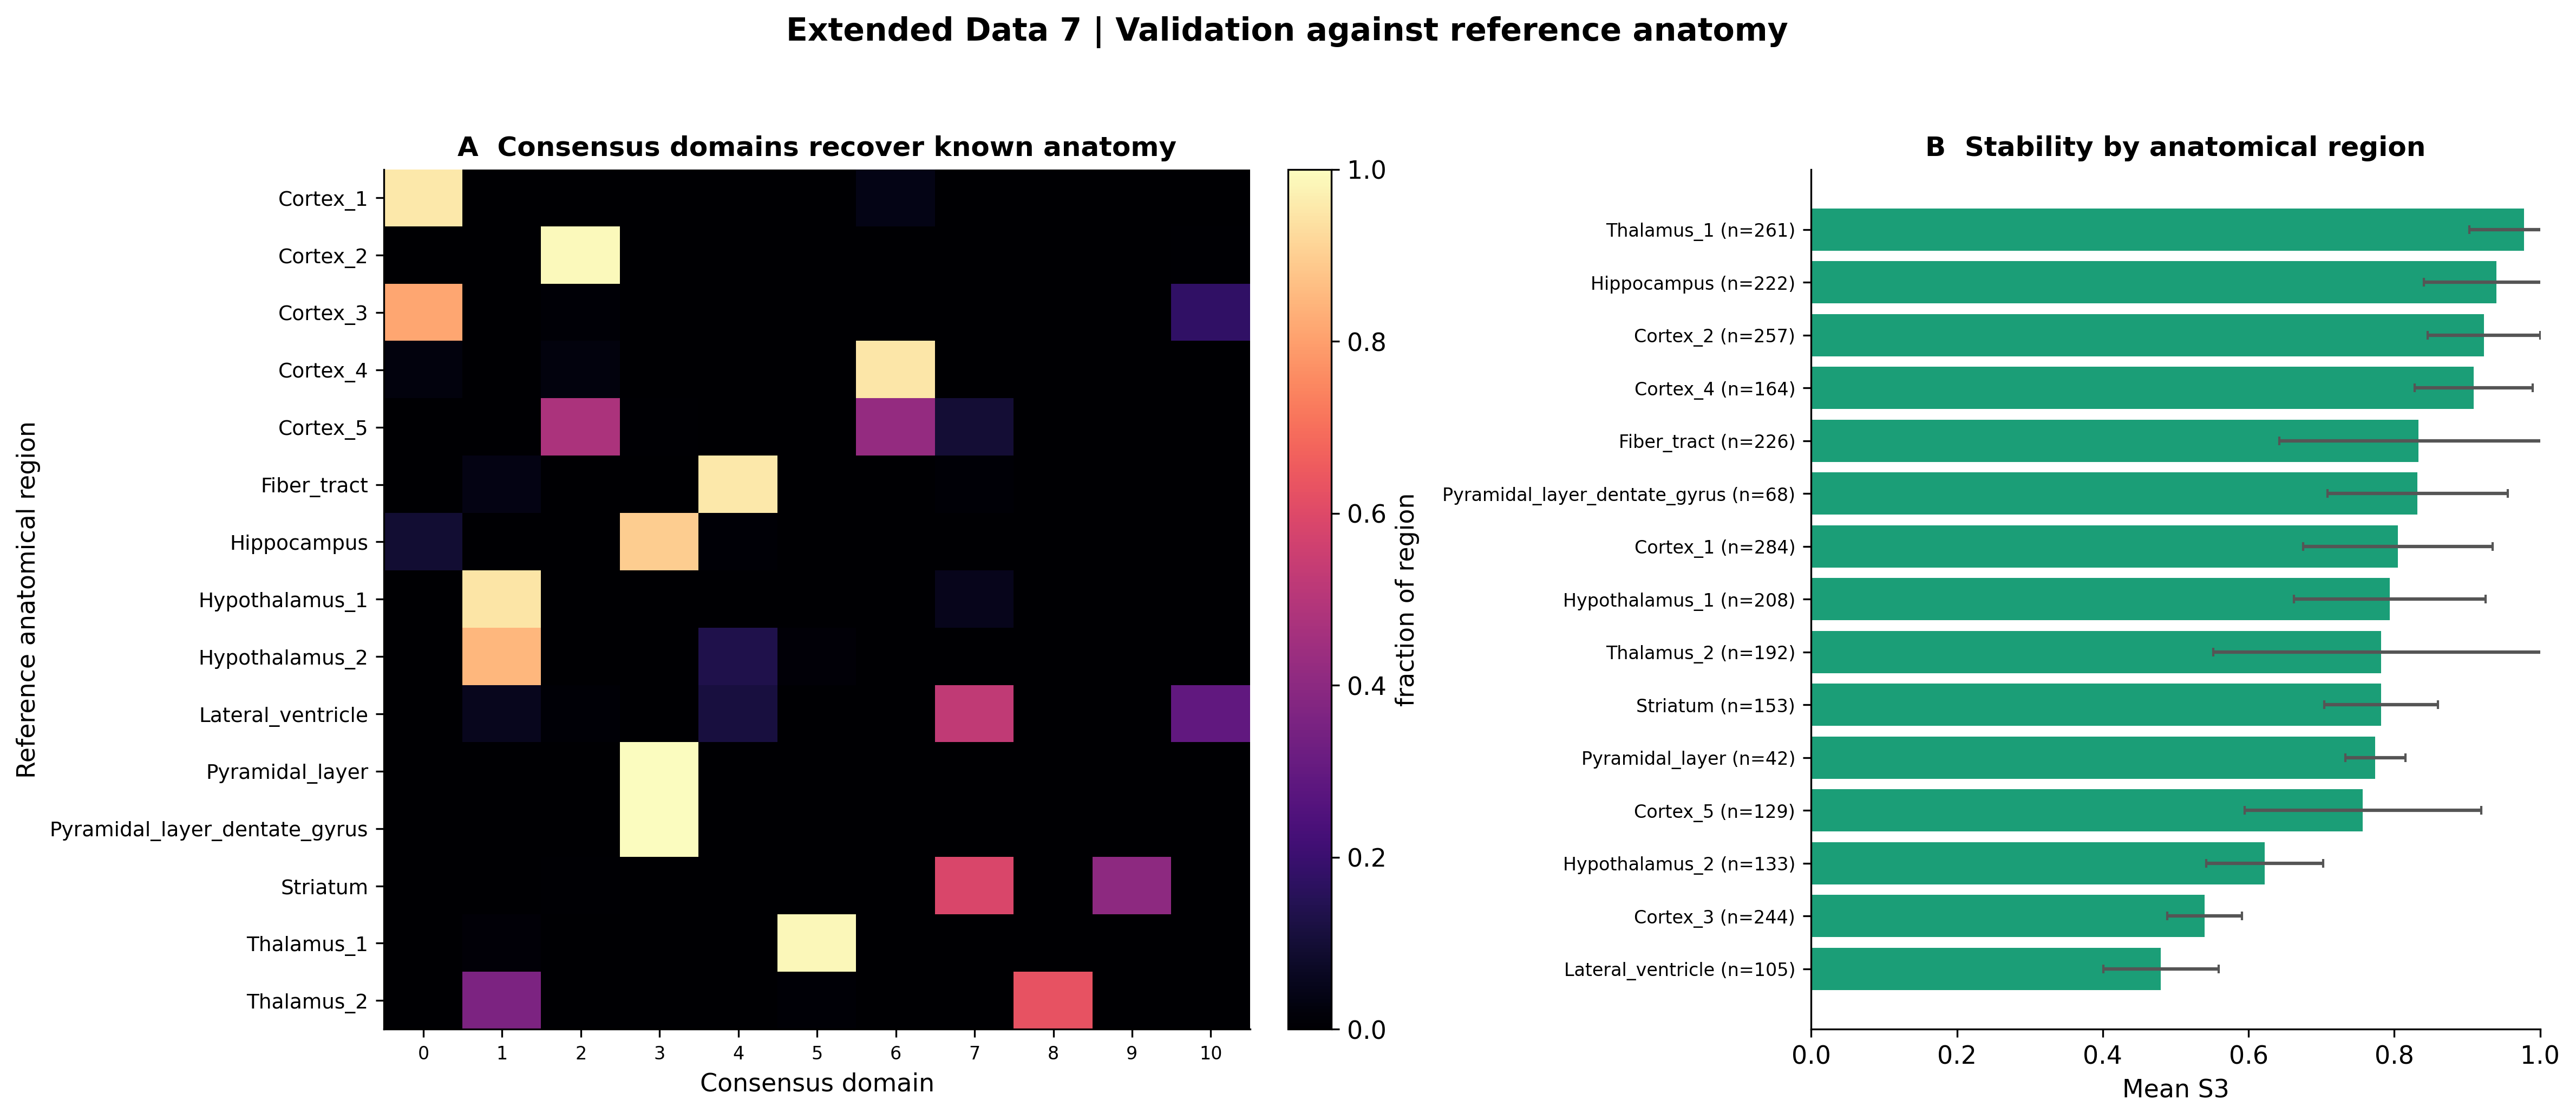
\includegraphics[width=\linewidth]{ed7_reference_validation.png}
  \caption{Extended Data: validation against the reference anatomy. (A) Row-normalized
  agreement between reference anatomical regions and multiverse consensus domains: each
  region maps predominantly to one domain, so the pipelines recover known structure.
  (B) Mean per-spot $S^3$ within each anatomical region: transcriptomically distinct
  structures (thalamus, hippocampus, cortical layers) are robust, while the lateral
  ventricle and mixed cortical zones are fragile.}
  \label{fig:refval}
\end{figure}

\begin{figure}[t]
  \centering
  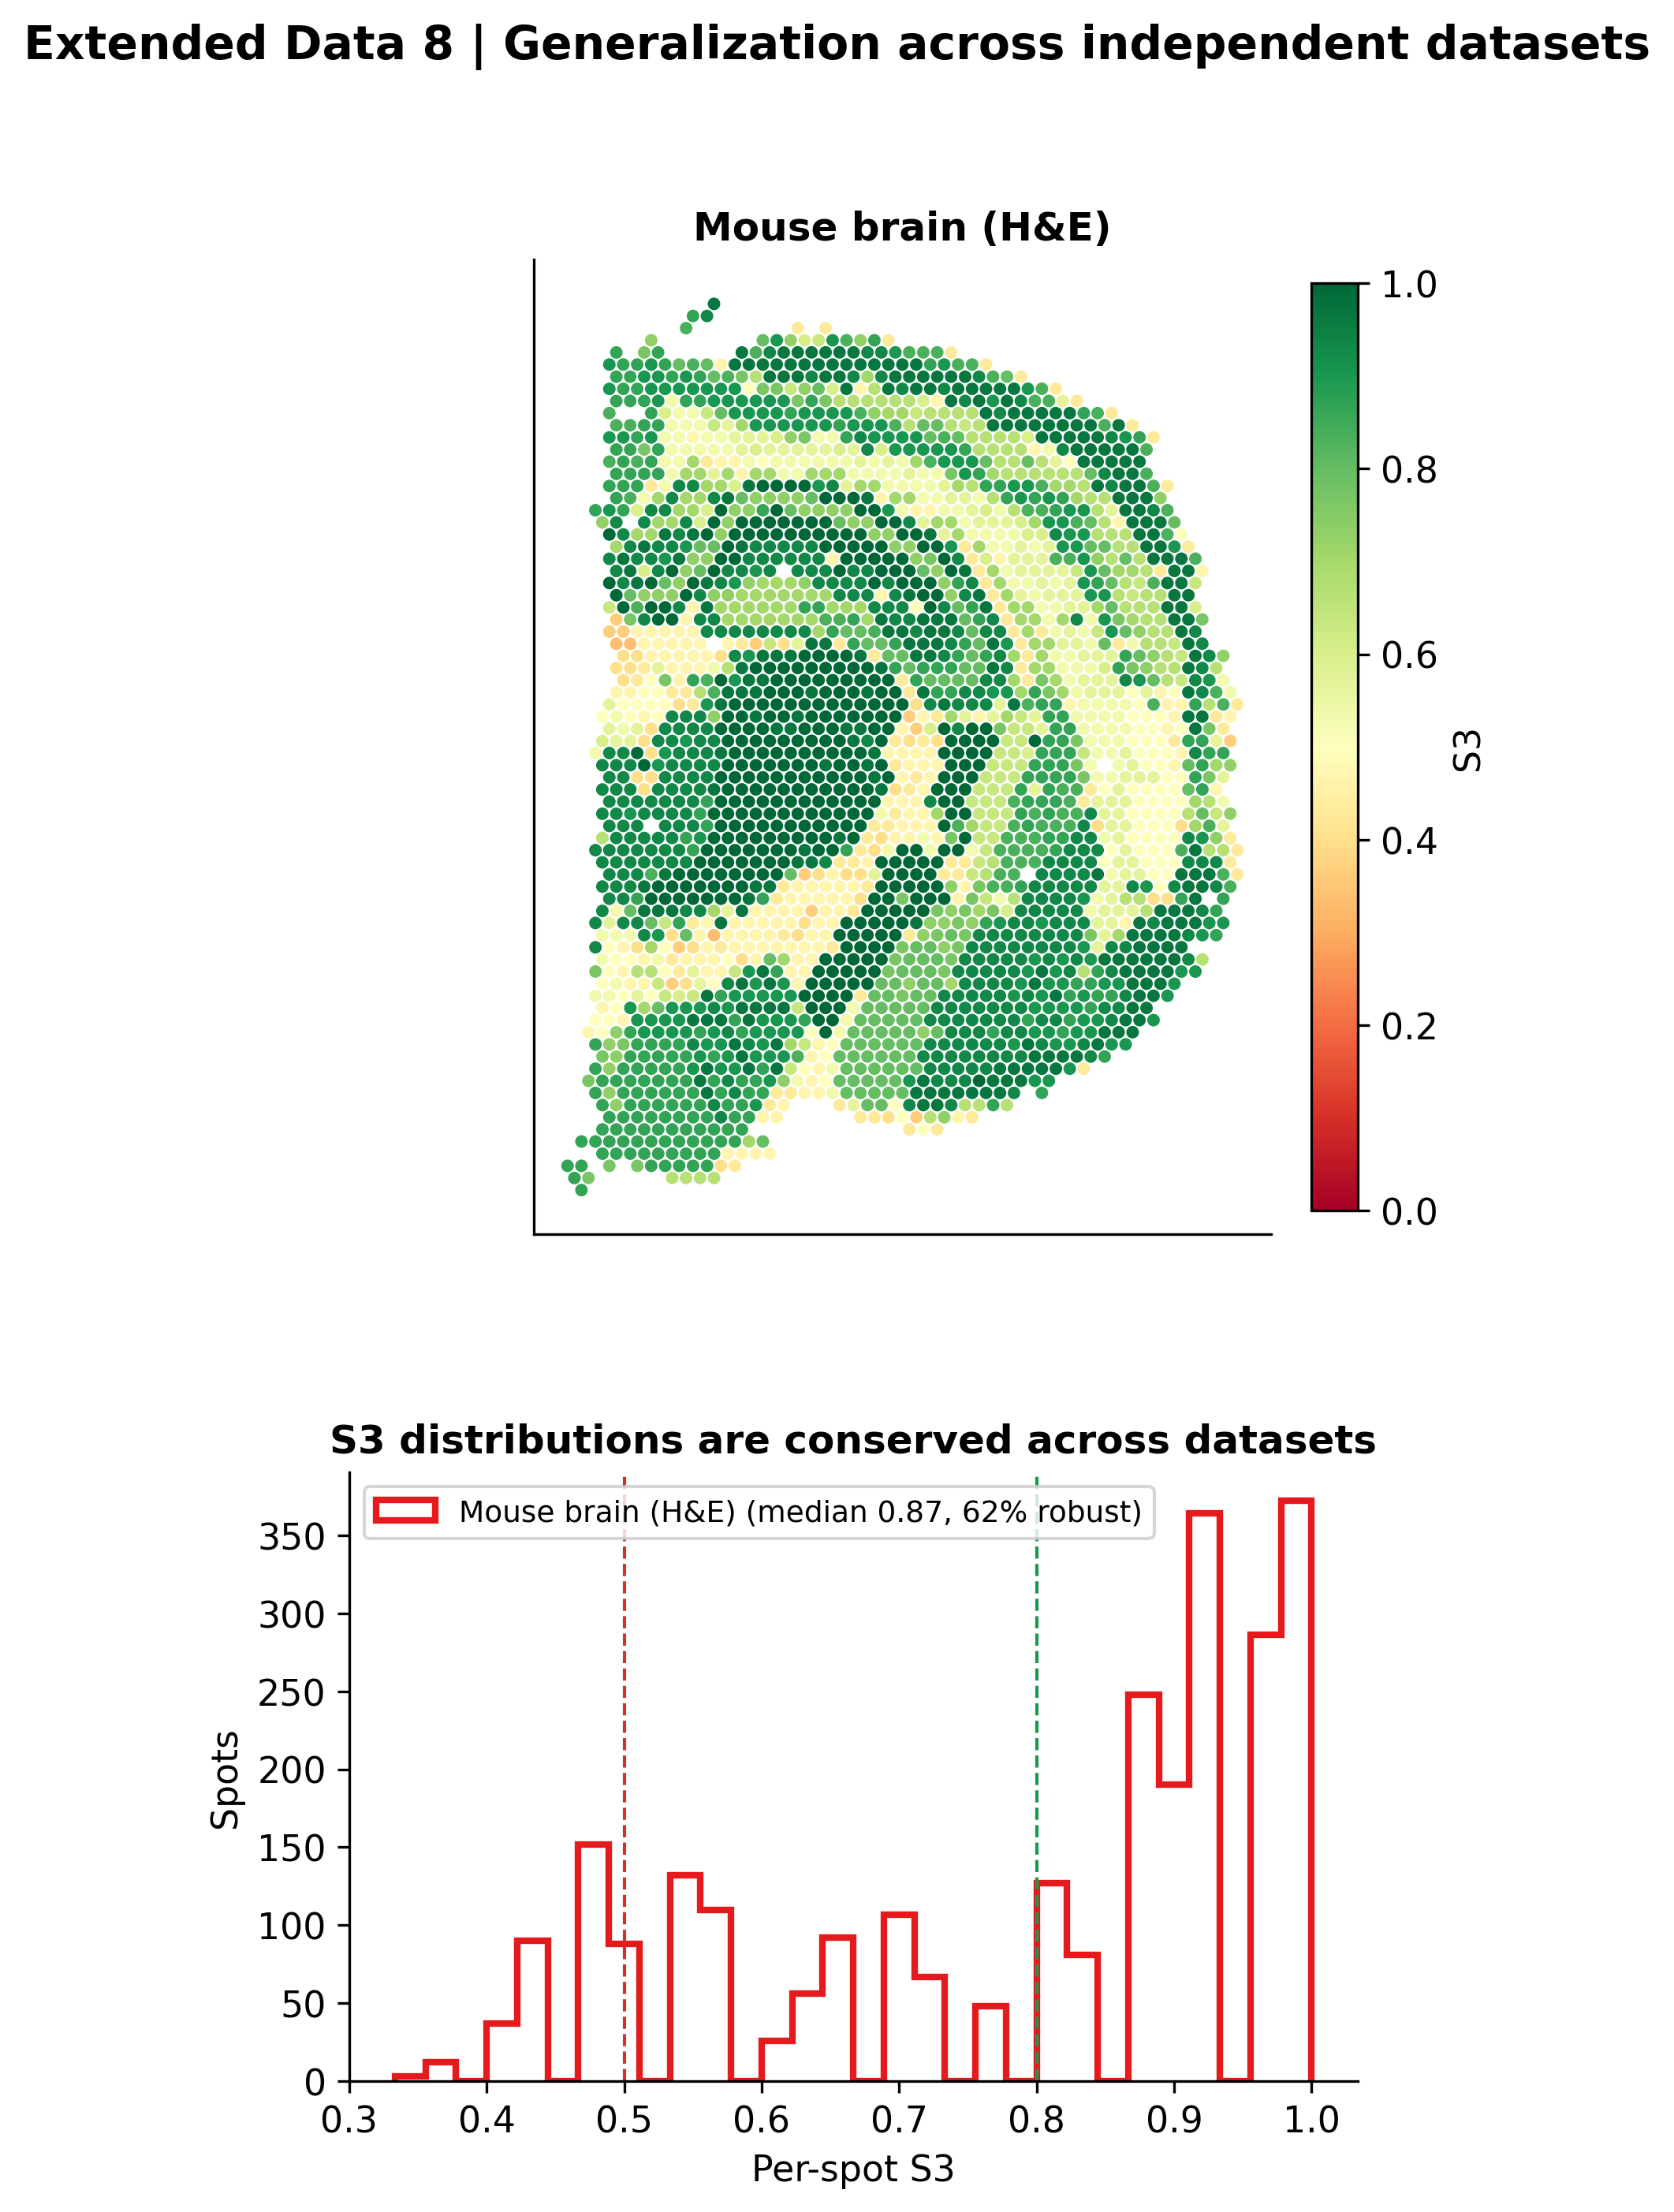
\includegraphics[width=\linewidth]{ed8_cross_dataset.png}
  \caption{Extended Data: generalization across independent datasets. Top: per-spot
  $S^3$ maps for two independently prepared mouse-brain sections (H\&E and
  fluorescence Visium). Bottom: their $S^3$ distributions are conserved (comparable
  medians and robust fractions), indicating the instability pattern is not specific to
  one slide.}
  \label{fig:cross}
\end{figure}

\begin{figure}[t]
  \centering
  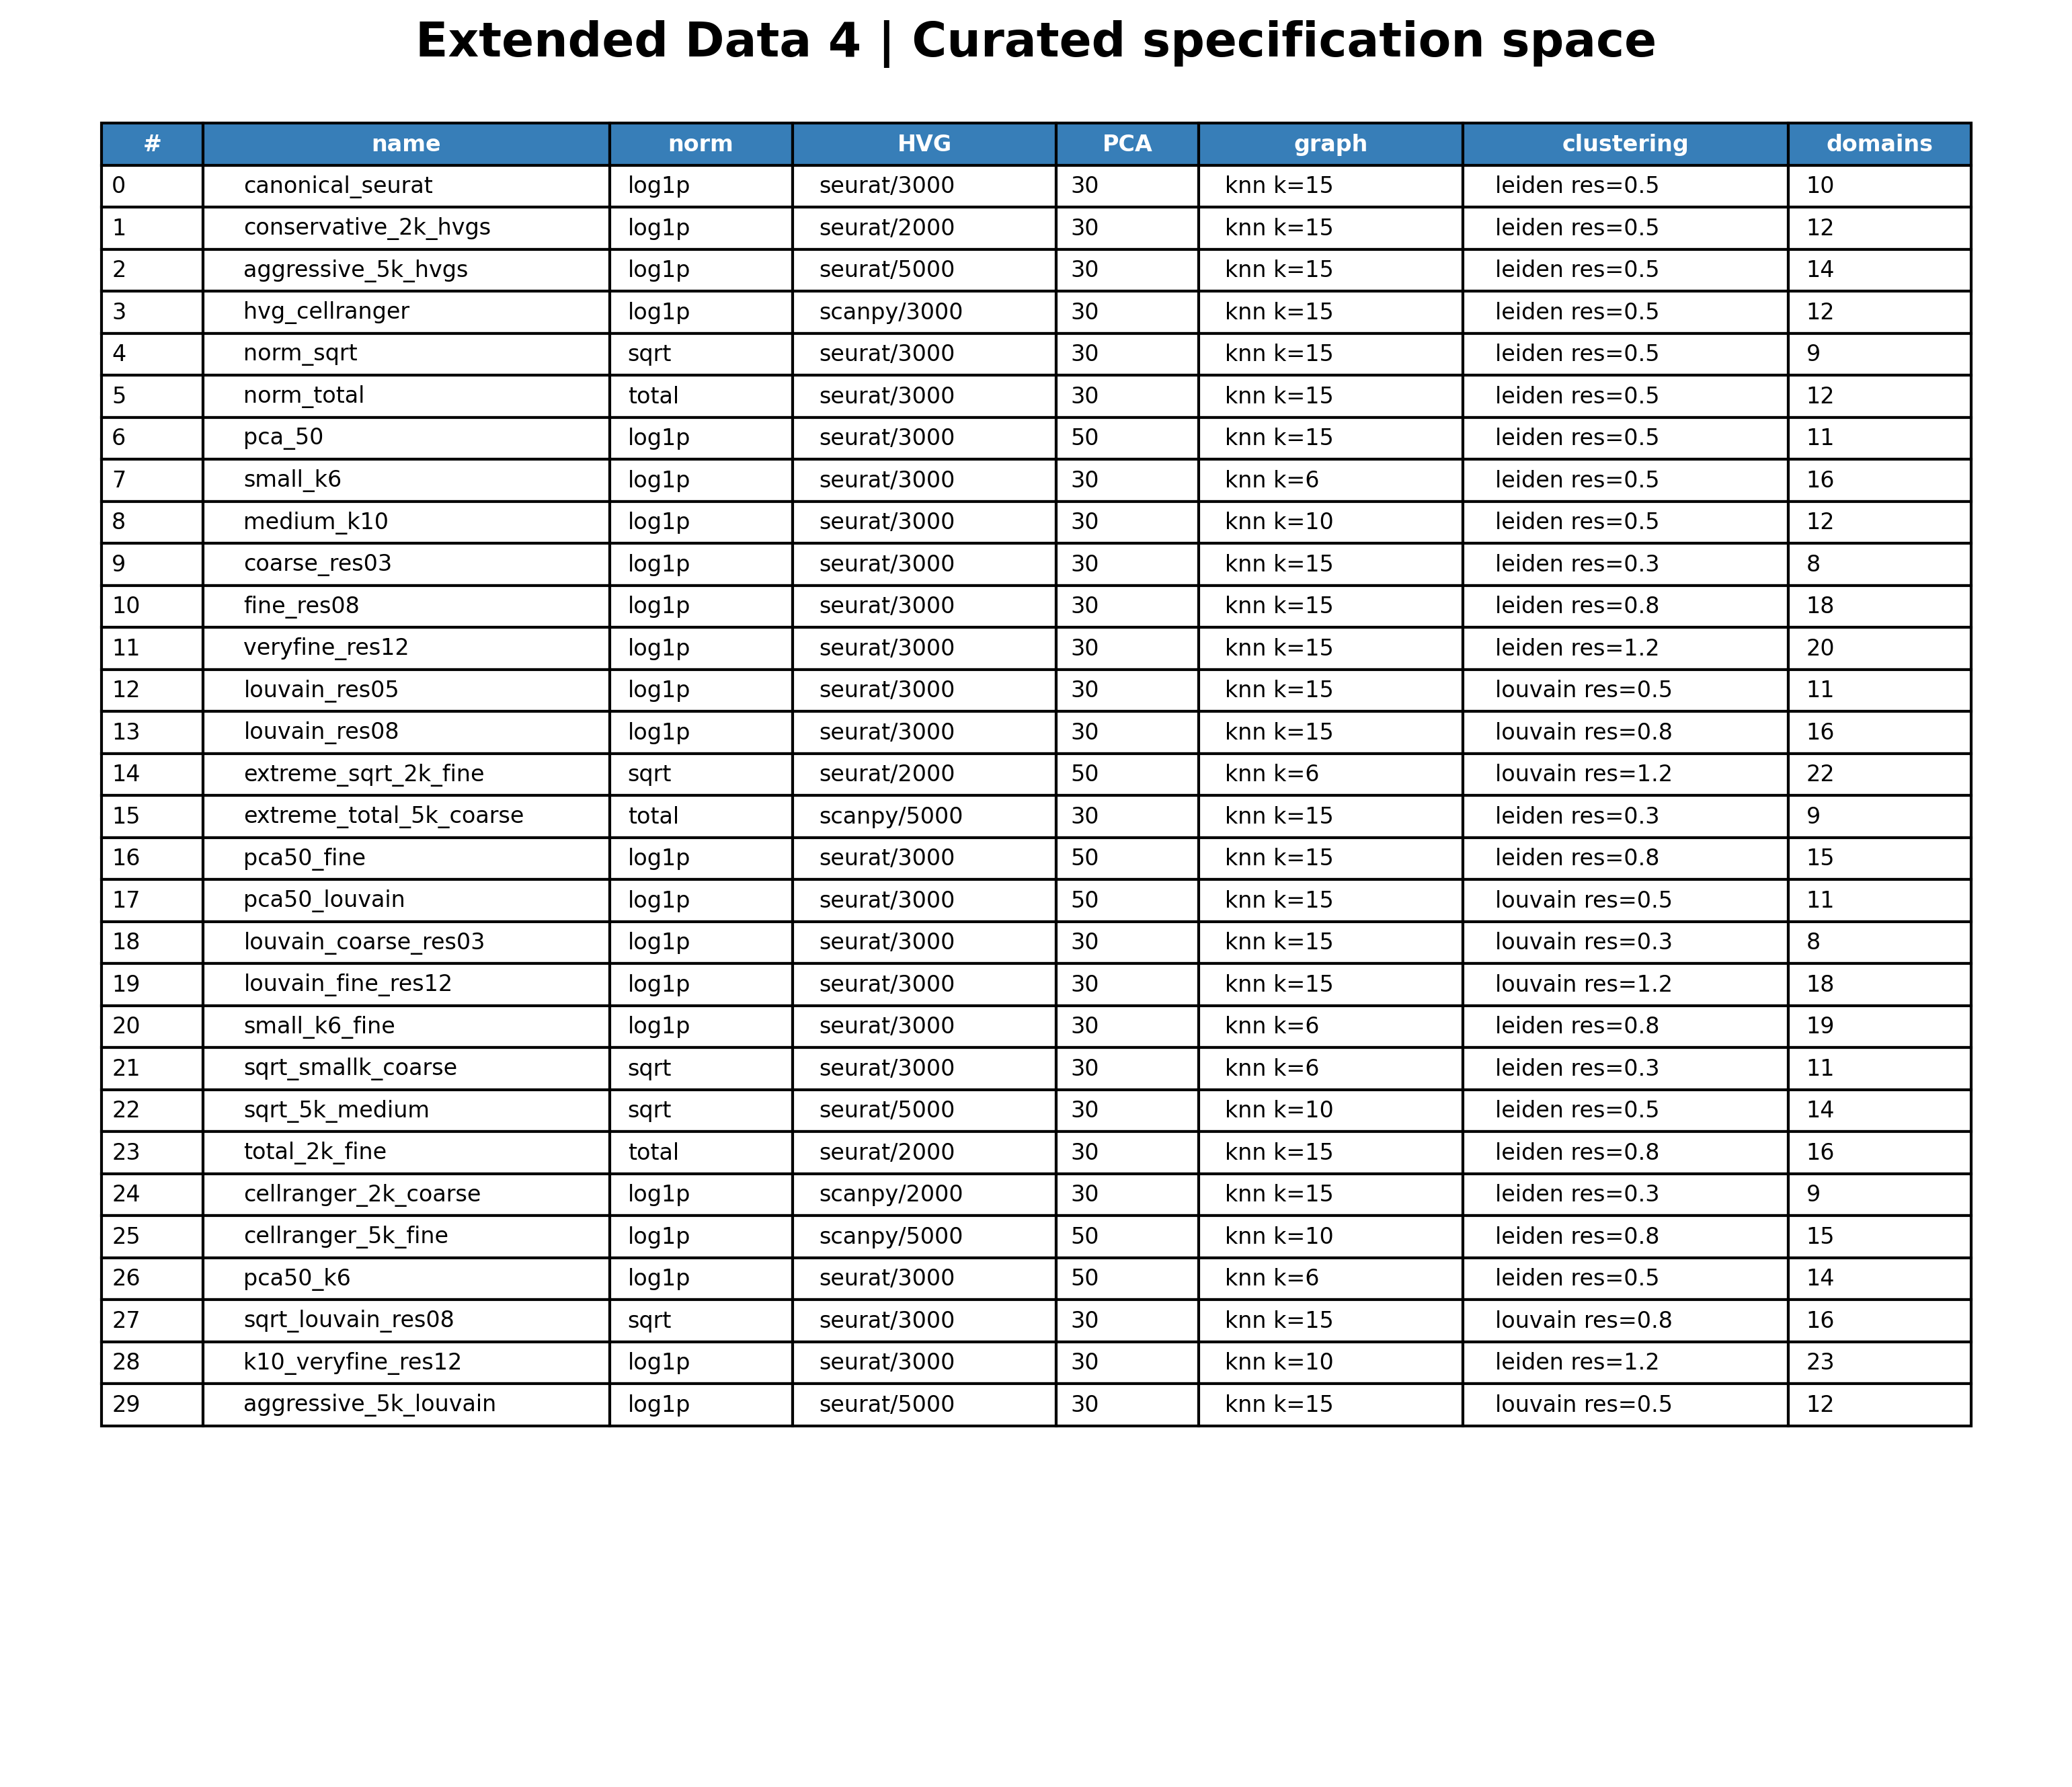
\includegraphics[width=\linewidth]{ed4_spec_space.png}
  \caption{Extended Data: the curated specification space. Each row is one of the
  \Nspecs{} pipelines with its analytical choices and resulting number of domains.}
  \label{fig:specspace}
\end{figure}

\begin{figure}[t]
  \centering
  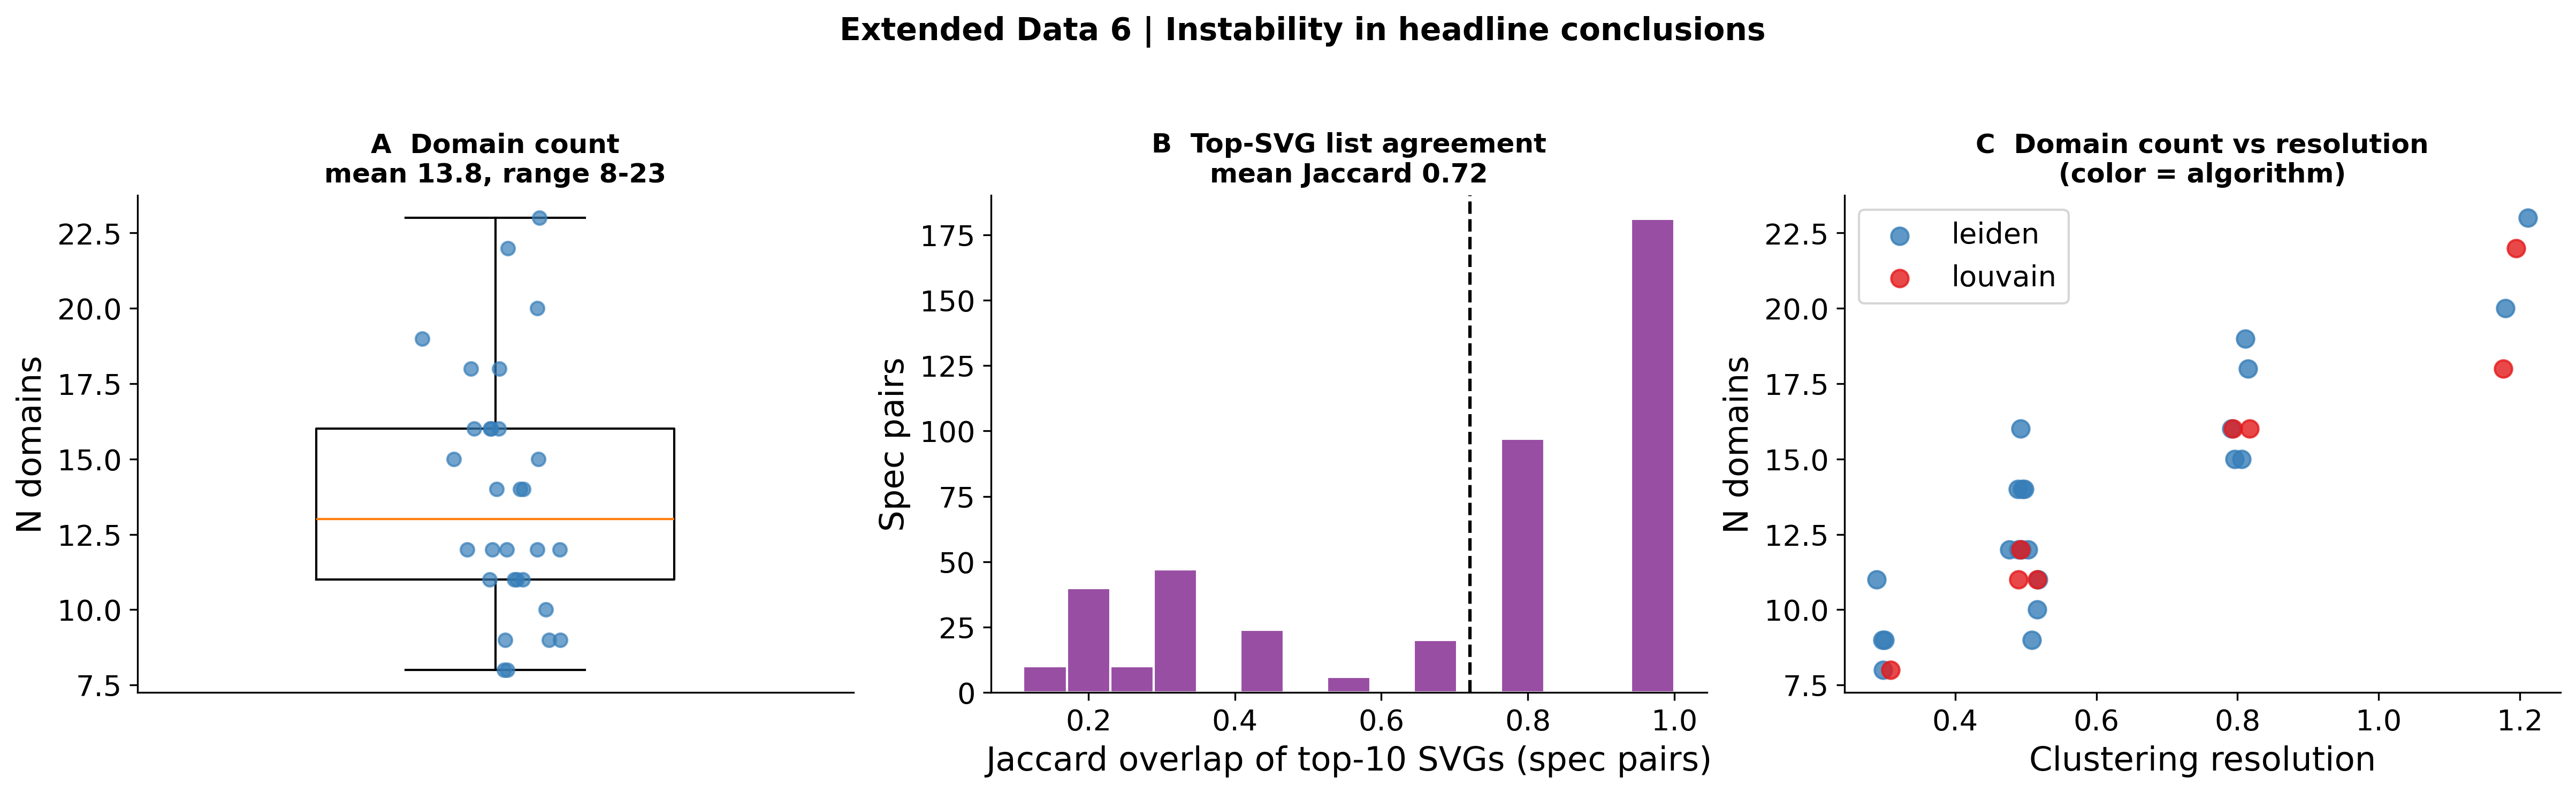
\includegraphics[width=\linewidth]{ed6_headline_instability.png}
  \caption{Extended Data: instability in headline conclusions. (A) Domain-count spread.
  (B) Jaccard overlap of top-10 SVG lists between specification pairs. (C) Domain count
  versus clustering resolution, split by algorithm---resolution is the dominant lever.}
  \label{fig:headline}
\end{figure}

\begin{figure}[t]
  \centering
  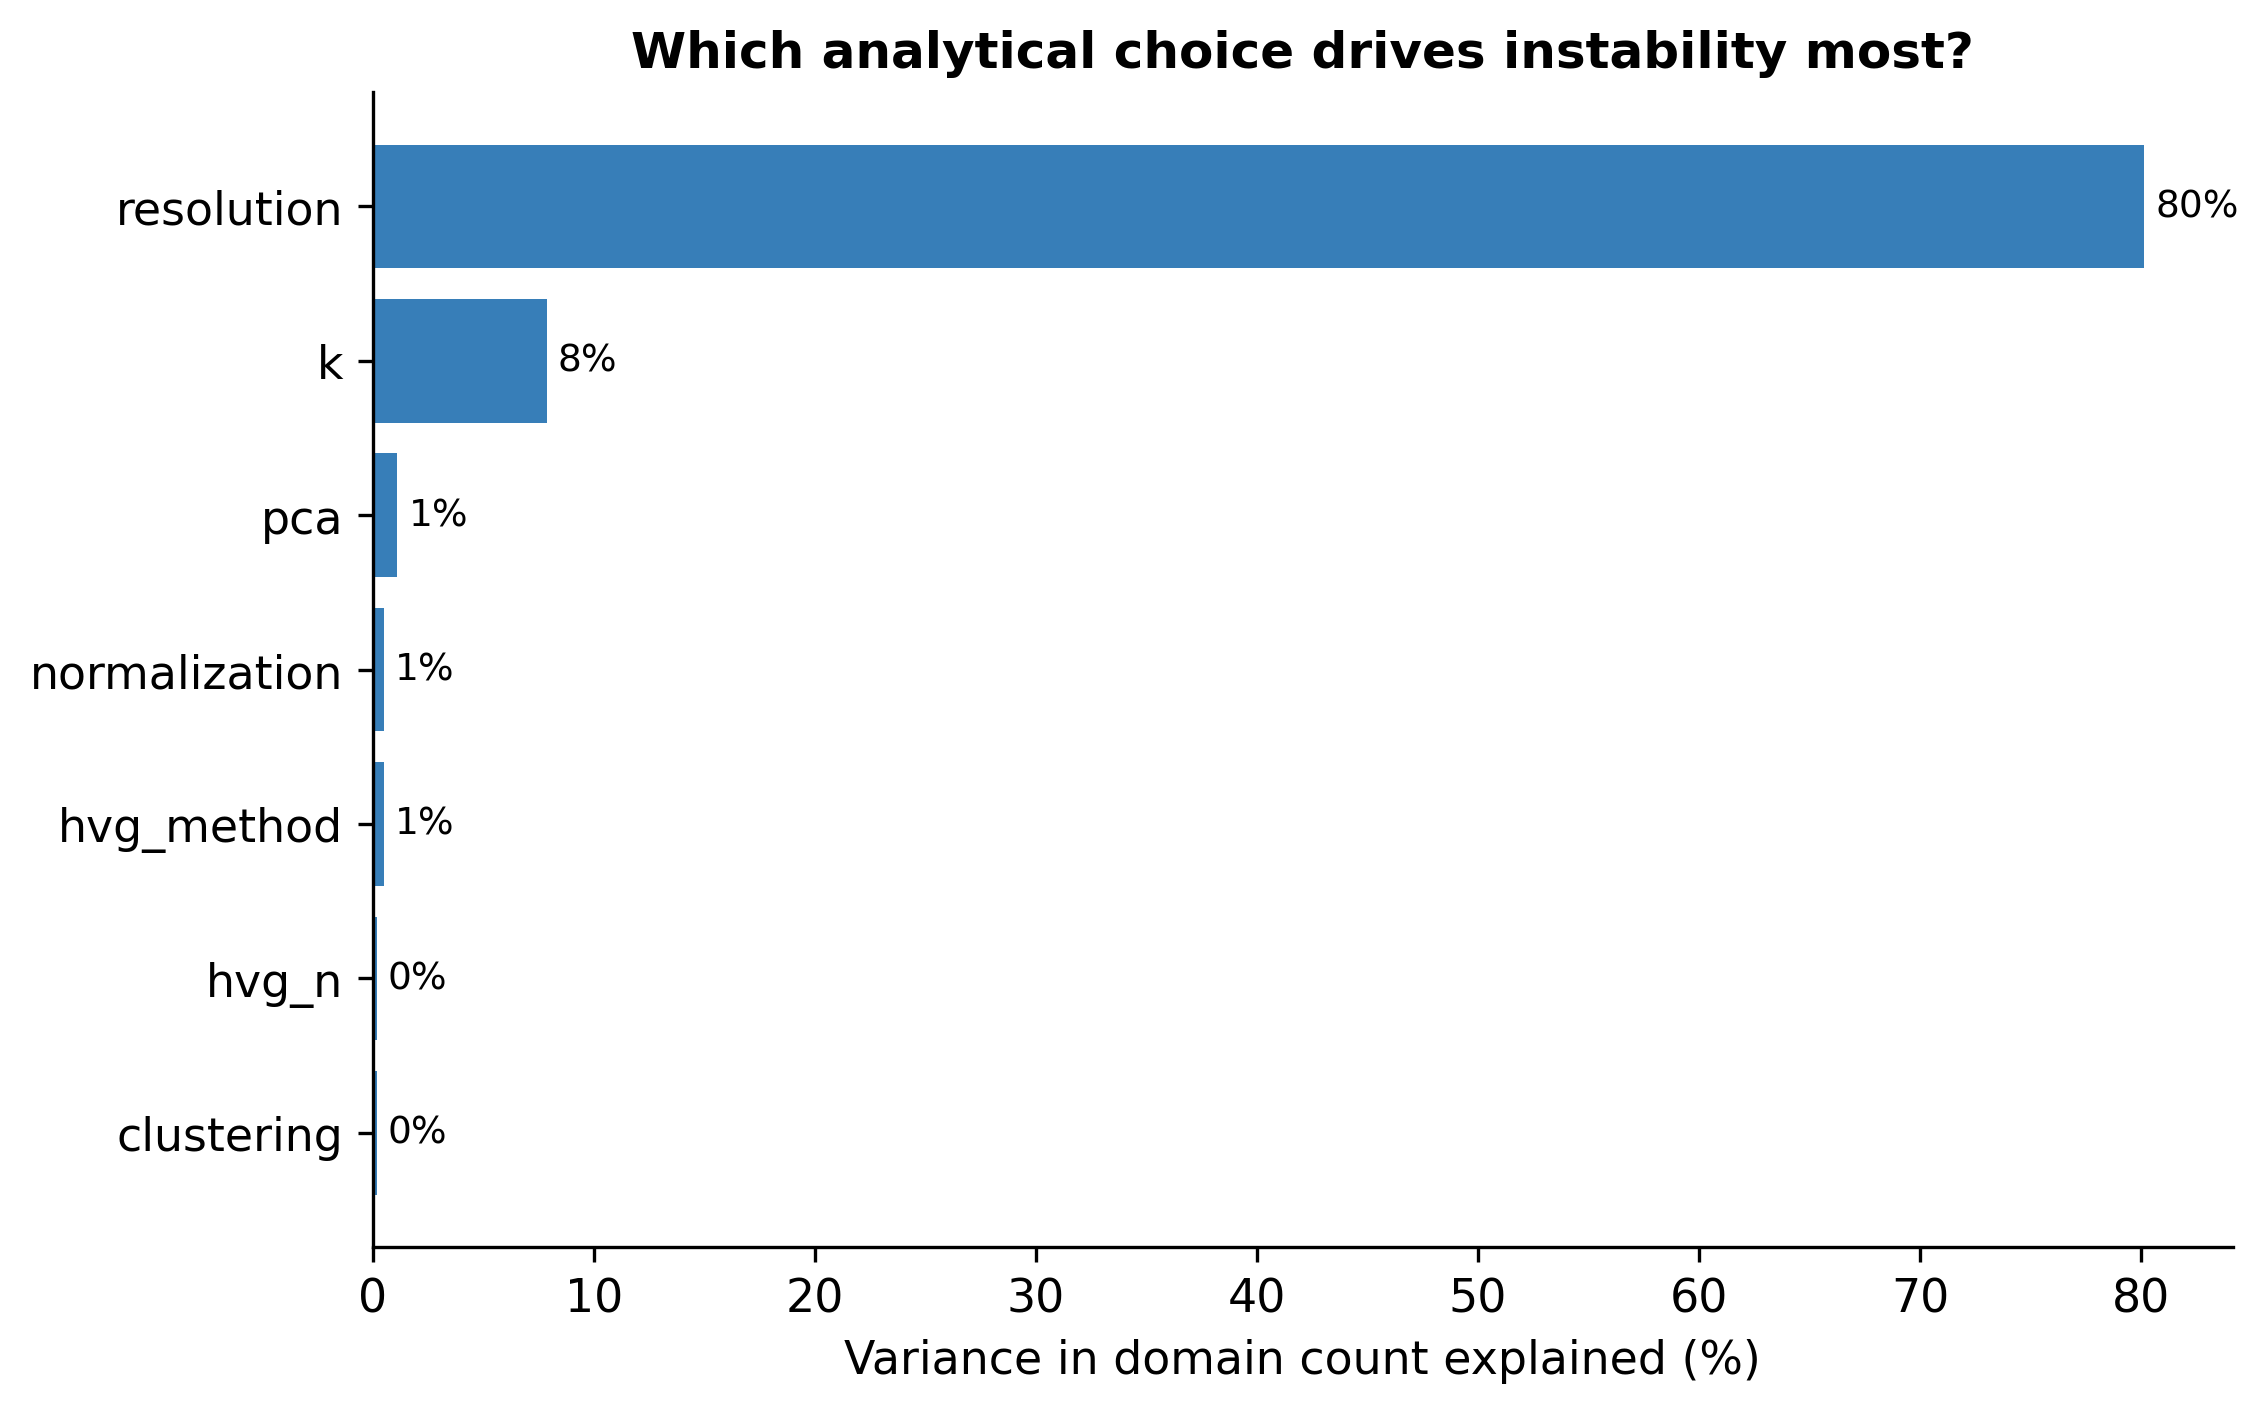
\includegraphics[width=0.75\linewidth]{08_variance_decomposition.png}
  \caption{Extended Data: variance in domain count attributed to each analytical axis
  (Type-II ANOVA). Clustering resolution dominates.}
  \label{fig:variance}
\end{figure}

\begin{figure}[t]
  \centering
  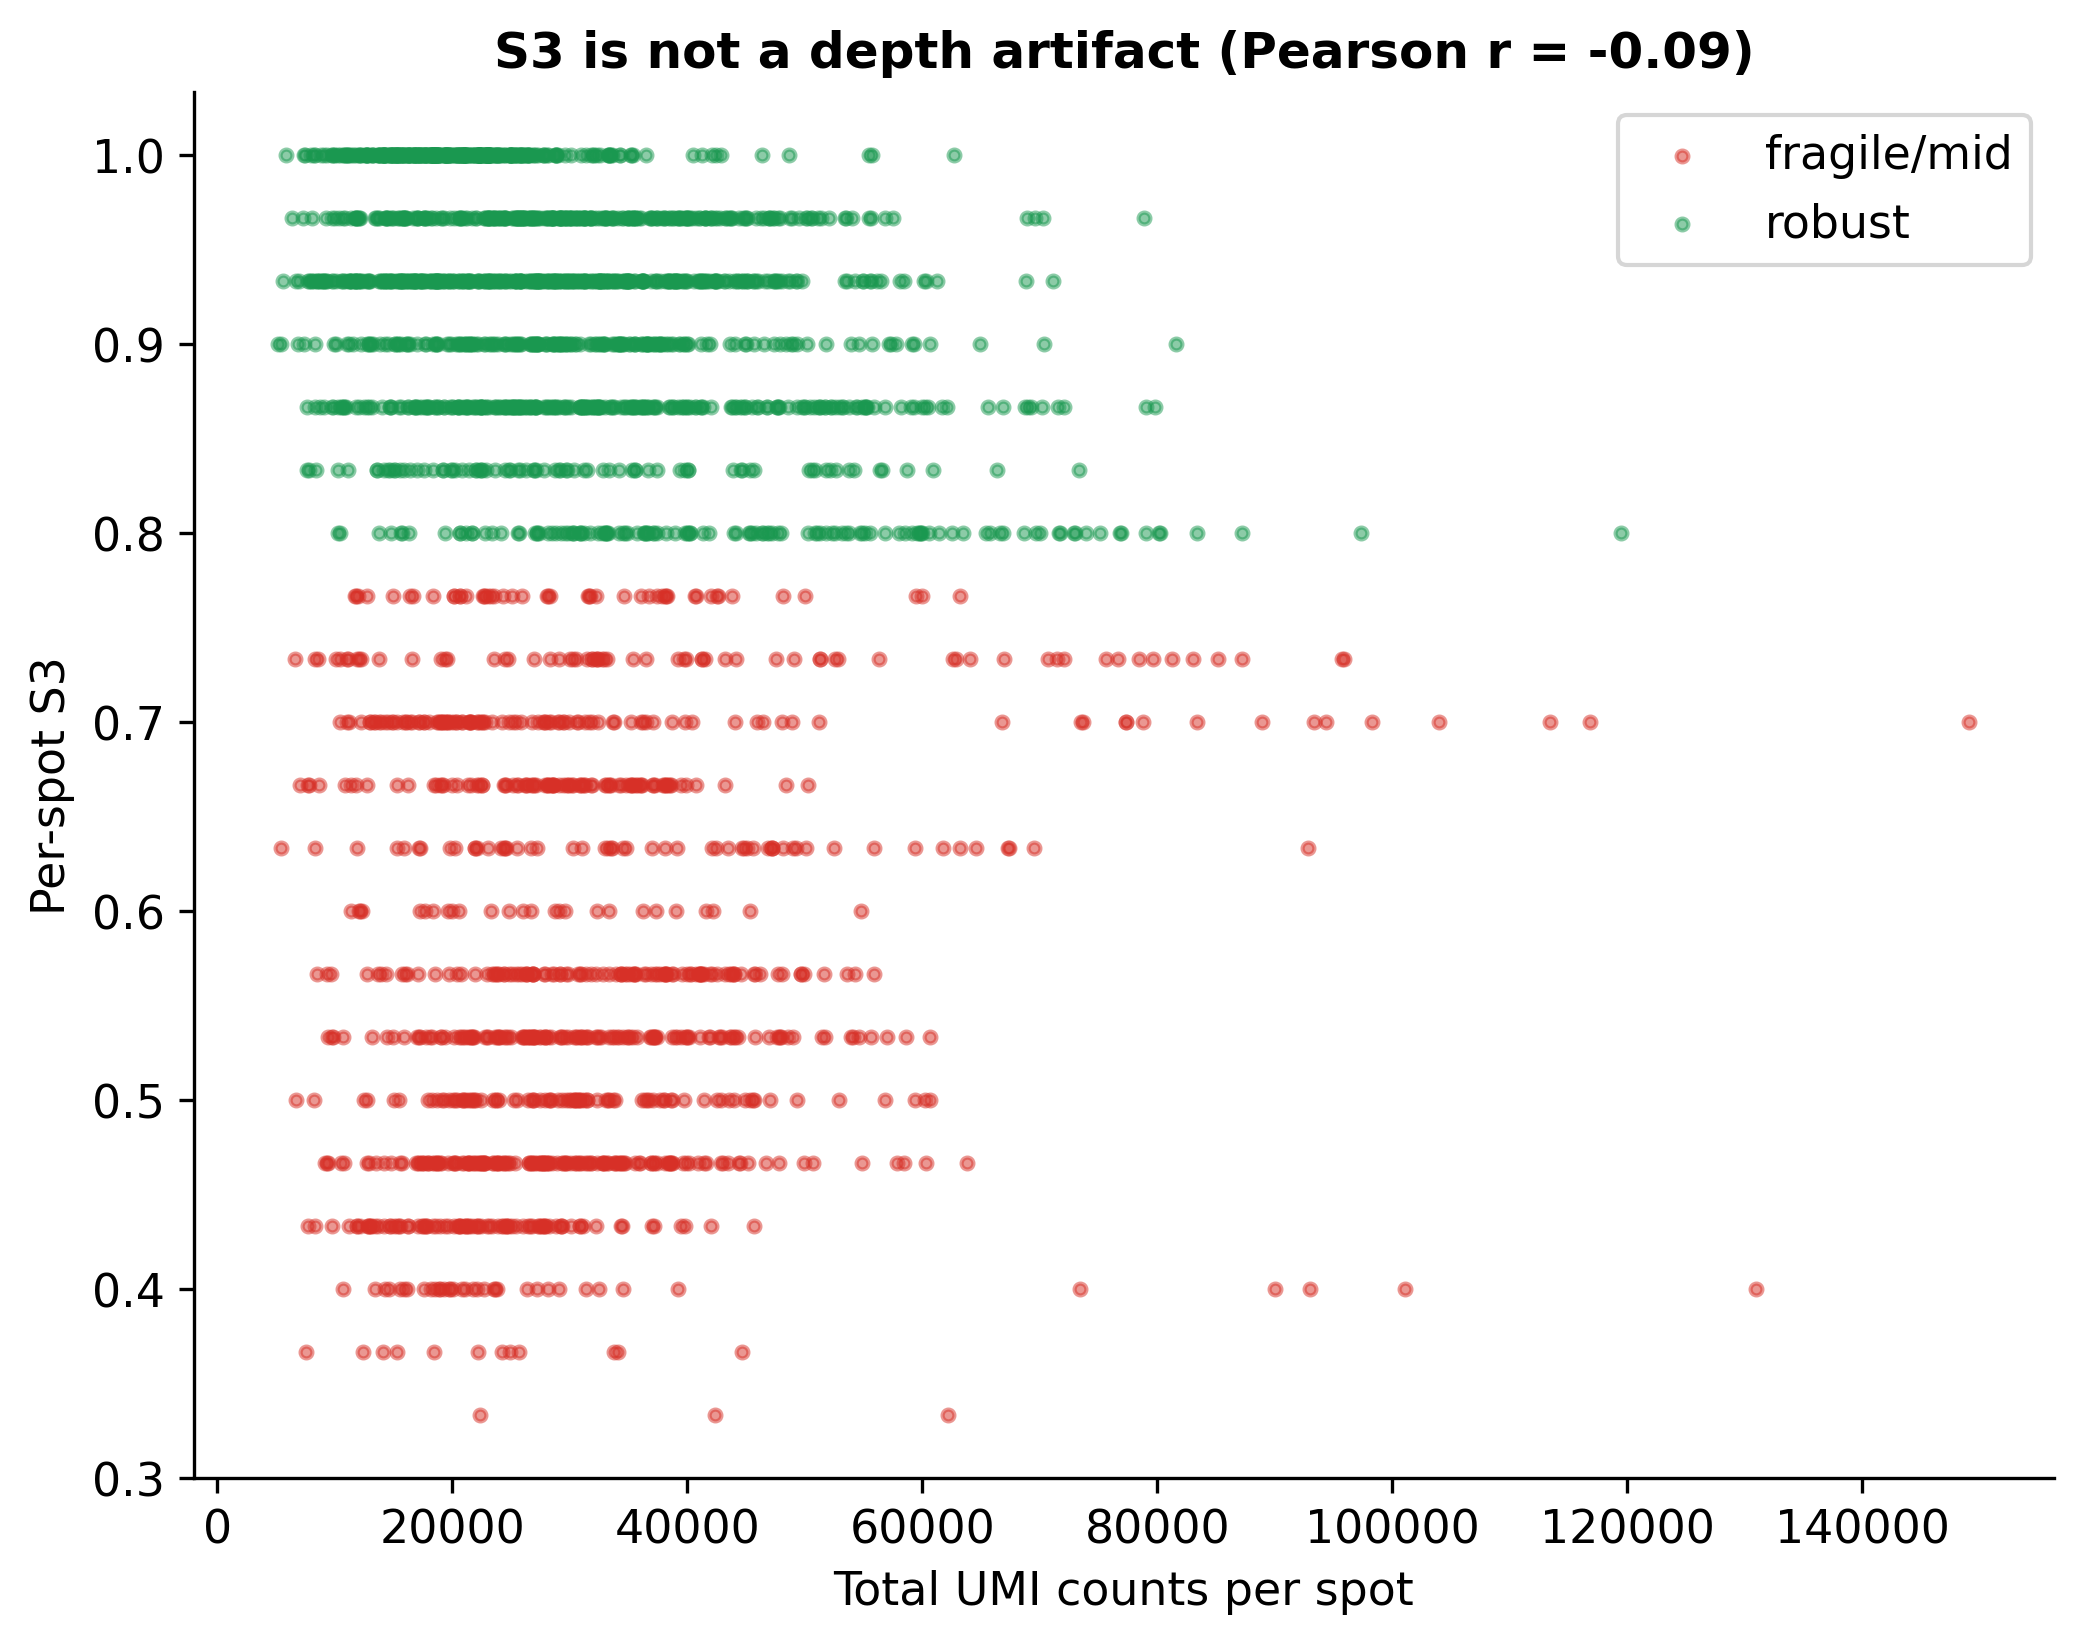
\includegraphics[width=0.7\linewidth]{11_confound_umi.png}
  \caption{Extended Data: per-spot $S^3$ versus total UMI counts. The near-zero
  correlation shows $S^3$ is not a proxy for sequencing depth; robust (green) and fragile
  (red) spots occur at all depths.}
  \label{fig:confound}
\end{figure}

\begin{figure}[t]
  \centering
  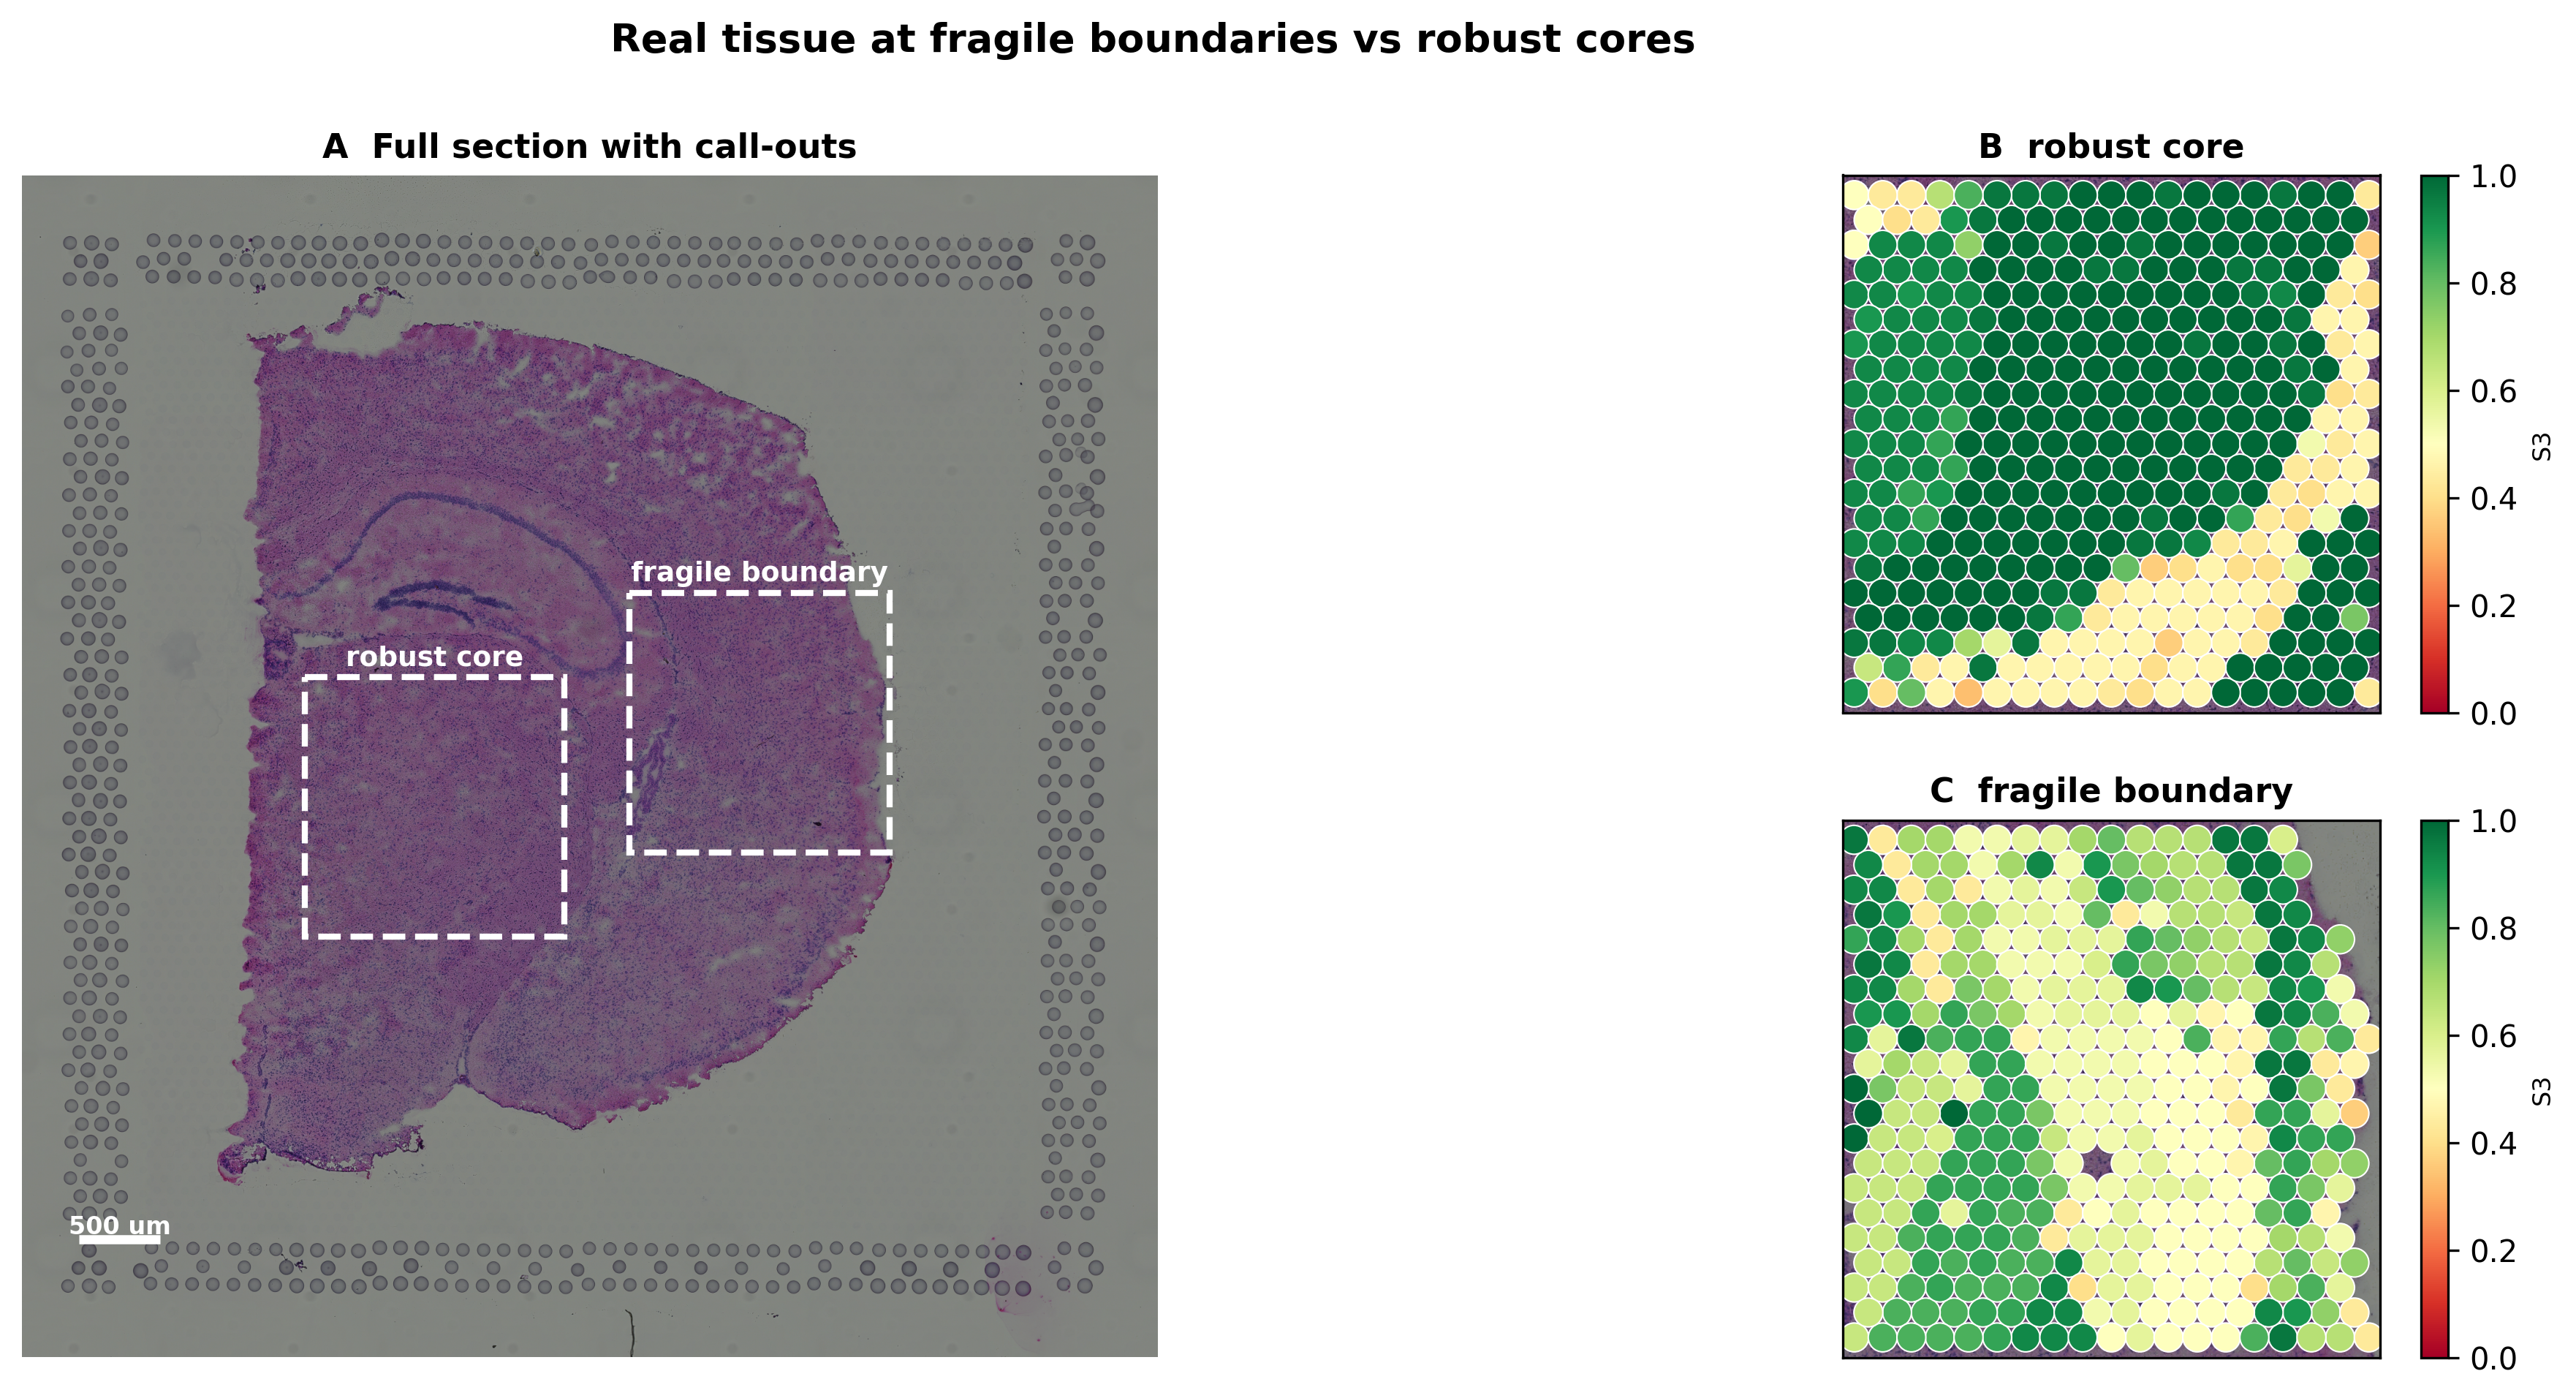
\includegraphics[width=\linewidth]{05_zoomed_insets.png}
  \caption{Extended Data: real H\&E tissue at a robust core versus a fragile boundary,
  with per-spot $S^3$ overlays. Fragile zones coincide with morphological transitions.}
  \label{fig:insets}
\end{figure}

\begin{figure}[t]
  \centering
  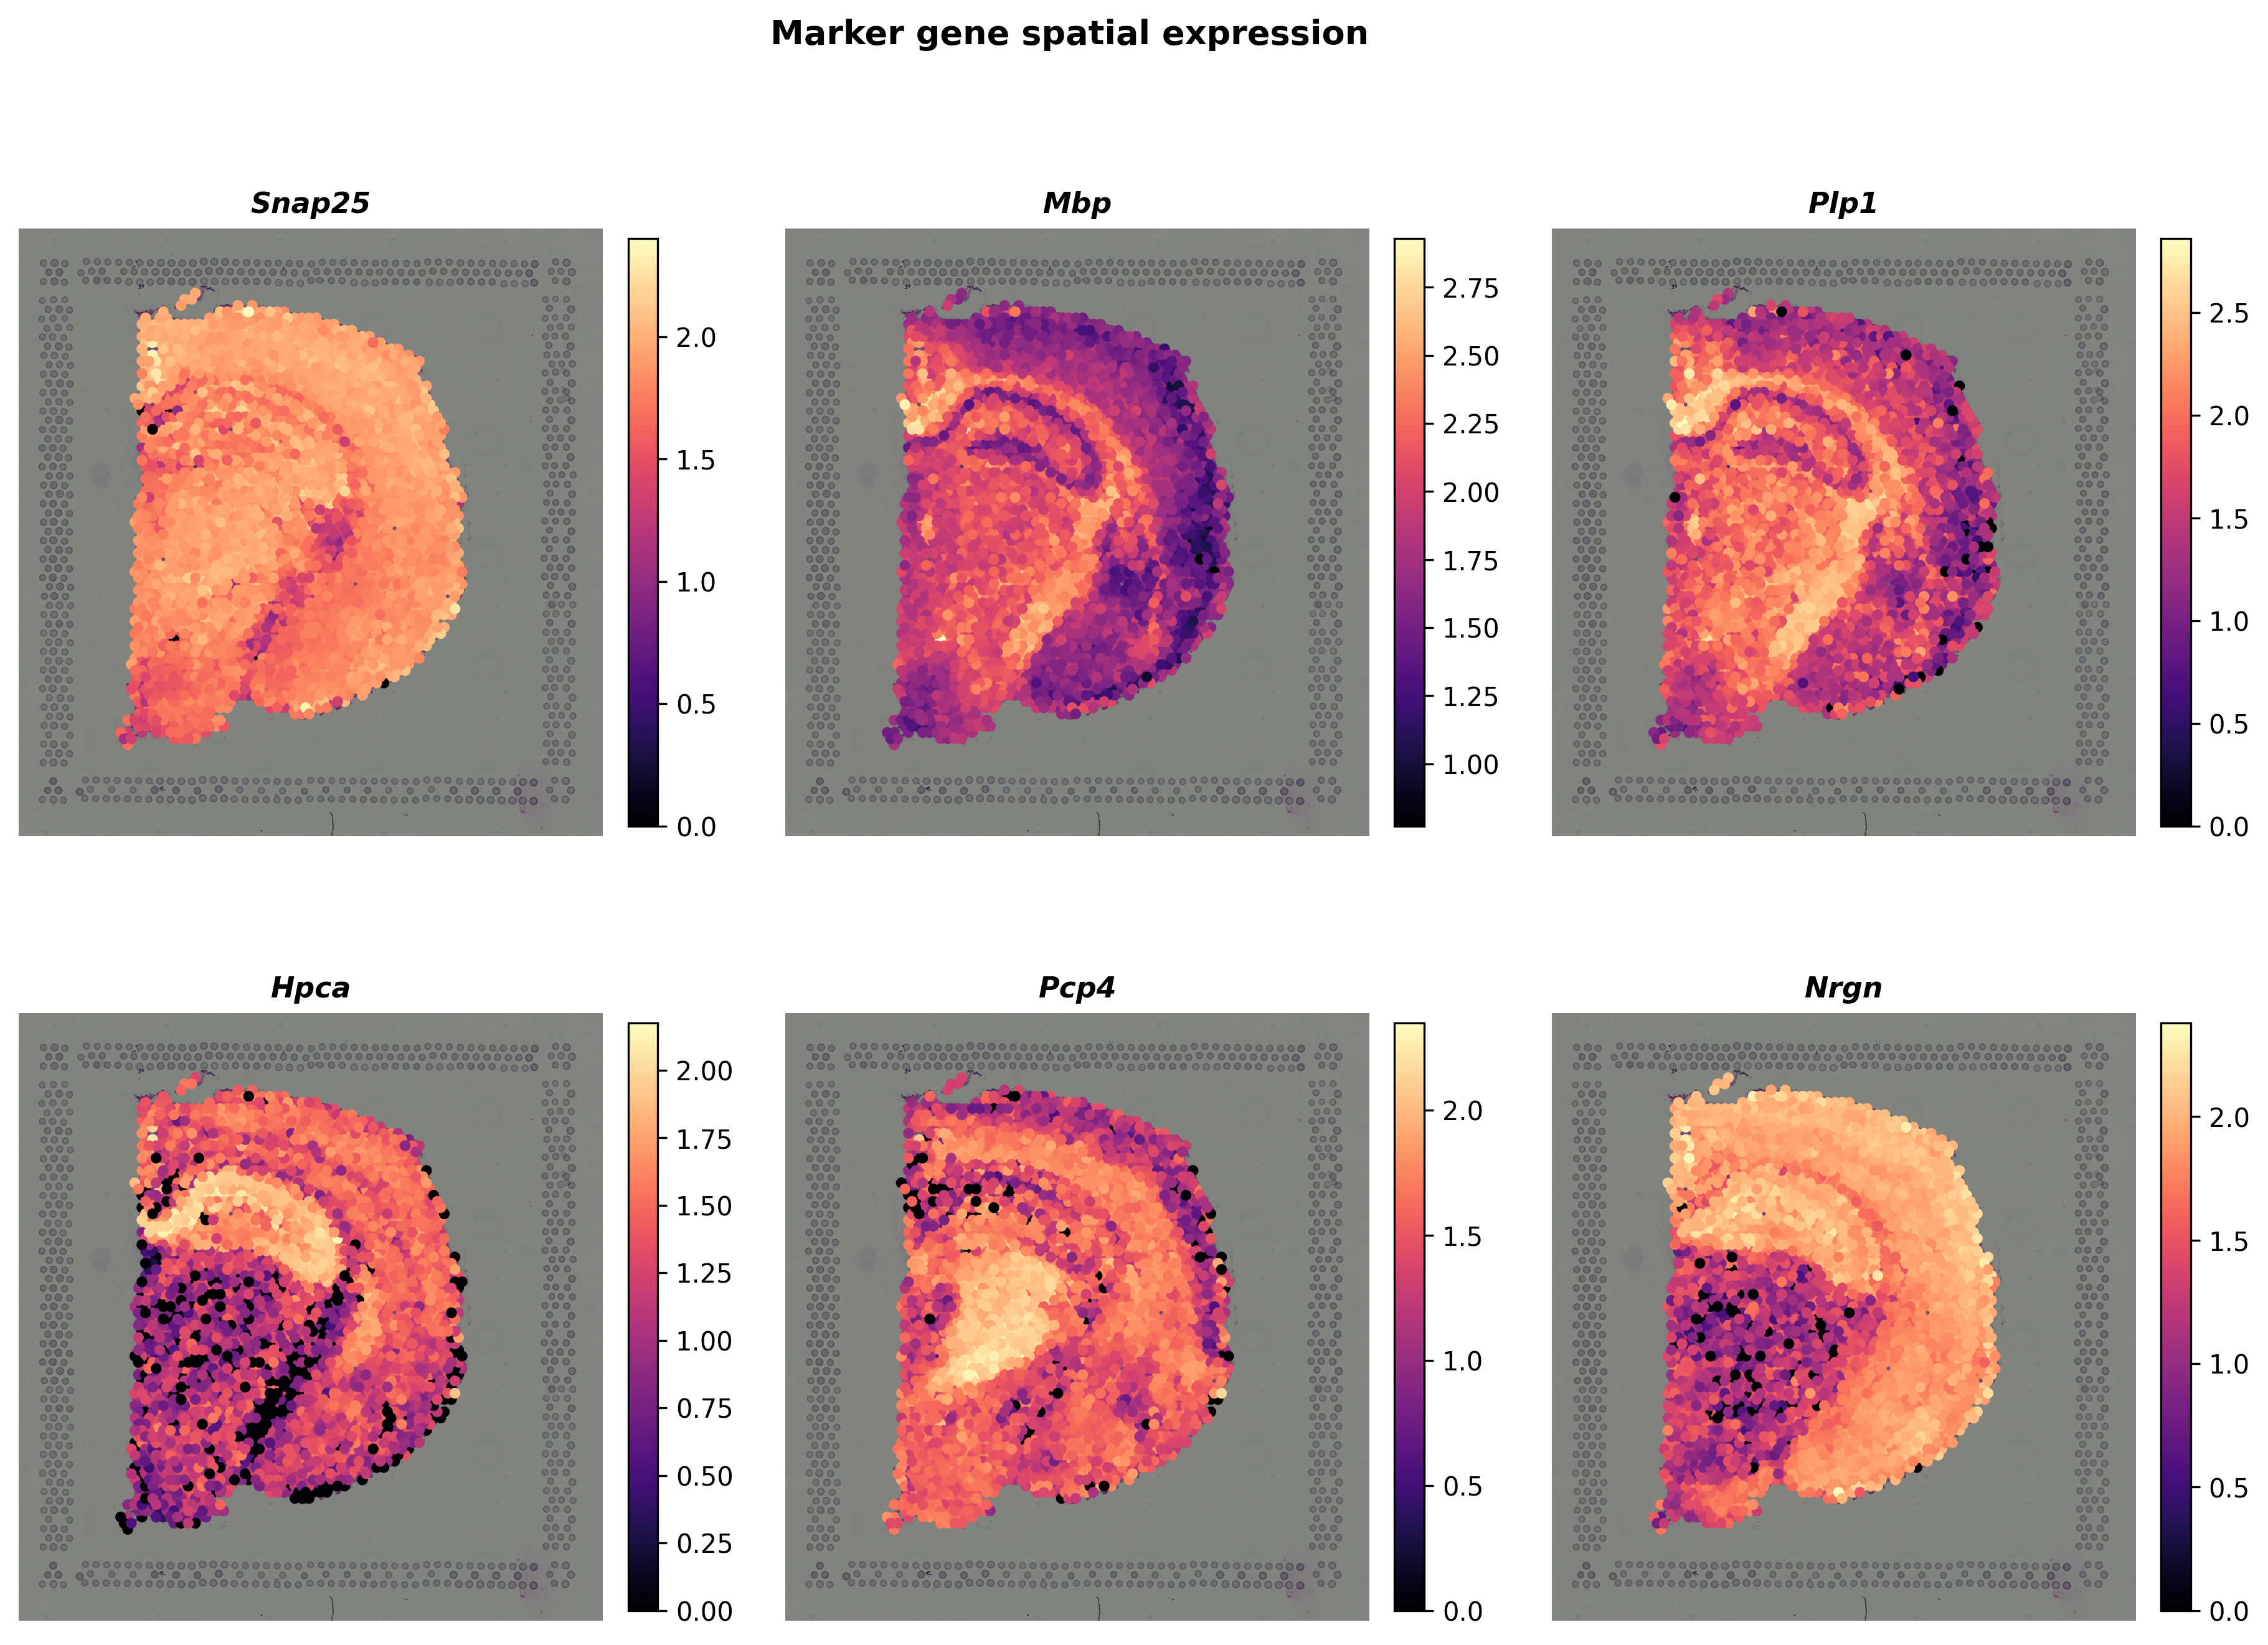
\includegraphics[width=\linewidth]{06_marker_genes.png}
  \caption{Extended Data: spatial expression of canonical mouse-brain markers on the
  H\&E image; the recovered patterns match known neuroanatomy (myelin in fiber tracts,
  \emph{Hpca} in hippocampus, \emph{Pcp4} in thalamus).}
  \label{fig:markers}
\end{figure}

\section{Practical Recommendations}
For researchers who cannot run a full multiverse, our variance decomposition
(Figure~\ref{fig:variance}) gives a concrete priority order. First, \emph{fix and report
the clustering resolution}: it accounts for \VarTopFrac{} of the variability in the number
of recovered domains, dwarfing every other choice. Second, report the neighborhood graph
size ($k$), the next largest contributor. Normalization, feature-selection method, HVG
count, PCA dimensionality, and the Leiden-versus-Louvain choice each move the result only
marginally and can be set to community defaults with little effect on the domain count.
Finally, treat spatially-variable-gene calls near the significance threshold as
provisional: they are the least reproducible conclusion across pipelines, and we recommend
reporting an $S^3$ per gene alongside any SVG list.

\section{Discussion and Limitations}
MOSAIC quantifies, rather than resolves, analytic ambiguity: it tells a researcher which
conclusions are robust and which are contingent, and provides a spatially-resolved map of
where to place trust. The agreement between per-spot $S^3$ and reference anatomy suggests
$S^3$ measures biological, not merely analytical, uncertainty. Limitations include the use
of a curated (not exhaustive) set of specifications, two mouse-brain Visium sections (a
broader survey across tissues and platforms such as Xenium remains future work), and a
single SVG test; the framework accommodates additional axes, datasets, and tests. Cross-pipeline label alignment is
heuristic, though the reported $S^3$ is robust to the choice of reference specification,
and our headline agreement metric (ARI) is label-free.

\section{Reproducibility}
Every specification is seeded and re-derives its inputs from raw counts. We release the
code, the specification configuration, the aggregate stability tables, and the figure
scripts; the entire study reproduces with \texttt{make repro}. Data are auto-downloaded
from public Squidpy mirrors.

\bibliographystyle{plainnat}
\bibliography{references}

\end{document}
